\documentclass[b5paper,10pt]{book}
\usepackage[spanish]{babel}
\usepackage[utf8]{inputenc}
%\usepackage{amsmath}
\usepackage{pslatex}
\usepackage[dvips]{graphicx}
\usepackage{amssymb}
\usepackage{hyperref}
\usepackage{makeidx}
%\usepackage[Sonny]{fncychap}


%\usepackage{graphicx,psfrag,floatflt,hyperref}
%\usepackage[footnote]{acronym}

\usepackage[cam,width=8.27in,height=11.69in,center,dvips,vorigin=-1in]{crop}
%------------------------------------------------------------------------------%
%PAGE MARGIN SETUP
%------------------------------------------------------------------------------%
\topmargin -0.5in
\headheight 14pt
\textheight 7.7in
\textwidth 6in
\oddsidemargin -0.5in
\evensidemargin -0.5in
\headsep 25pt
\parskip 10pt

\makeindex


\begin{document}

\begin{titlepage}
\title{\centering \fontsize{28}{28} \selectfont Conceptos Básicos\\ de Geoestadística}
%\thanks{Profesor a cargo Daniel Villa, ayudante de la Evangelina Giuriati.}
\author{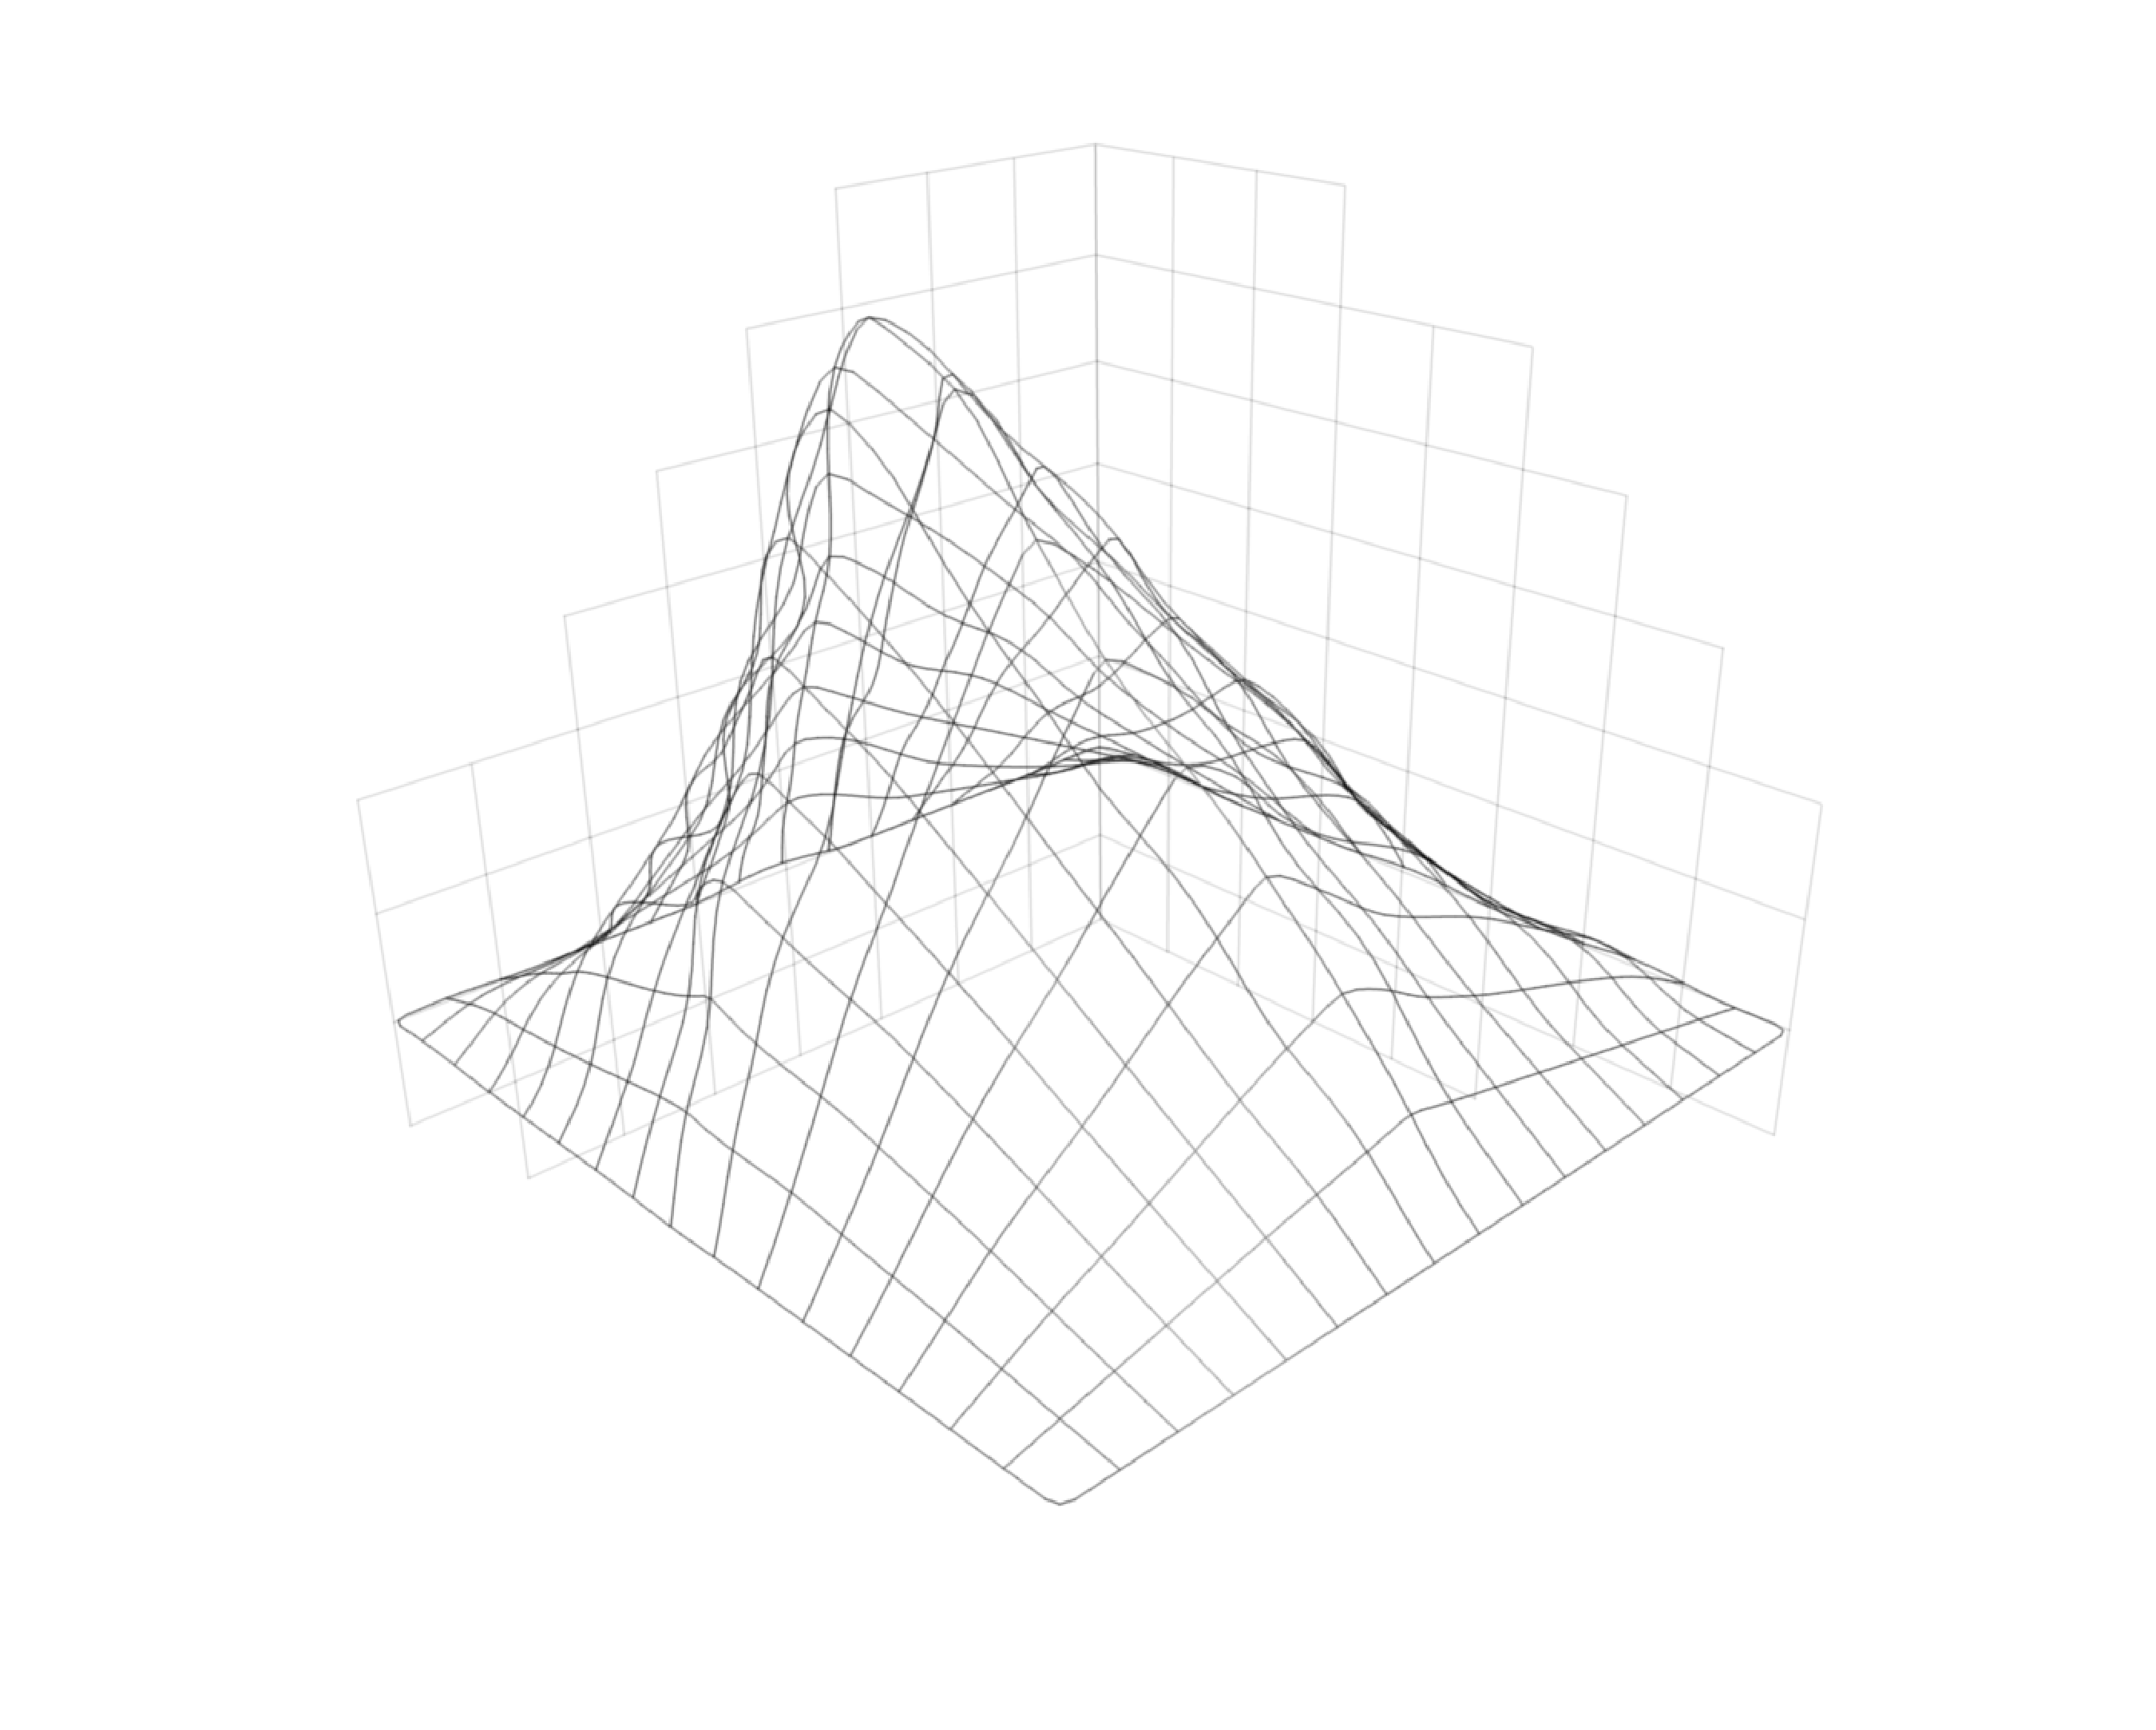
\includegraphics[scale=0.28]{image/logo.eps}\vspace*{1in}\\Eloy Colell \hfill Juan Uribe \hfill Pablo Chale}
\date{}
\maketitle
\thispagestyle{empty}
\end{titlepage}

\begin{titlepage}
\begin{figure}[b]
{\centering \fontsize{18}{18} \selectfont Conceptos Básicos de Geoestadística}
\\

Editado por

Lucas Capalbo Lavezzo.
\end{figure}
\end{titlepage}

% <a rel="license" href="http://creativecommons.org/licenses/by-nc-nd/3.0/"><img alt="Creative Commons License" style="border-width:0" src="http://i.creativecommons.org/l/by-nc-nd/3.0/88x31.png" /></a><br /><span xmlns:dc="http://purl.org/dc/elements/1.1/" href="http://purl.org/dc/dcmitype/Text" property="dc:title" rel="dc:type">Conceptos Básicos de Geoestadística</span> by <span xmlns:cc="http://creativecommons.org/ns#" property="cc:attributionName">Eloy Colell, Juan Uribe, Pablo Chale</span> is licensed under a <a rel="license" href="http://creativecommons.org/licenses/by-nc-nd/3.0/">Creative Commons Attribution-NonCommercial-NoDerivs 3.0 Unported License</a>.

\begin{titlepage}

\vspace*{5in}

\begin{figure}[b]
\includegraphics[clip, scale=1]{image/by-nc-nd.eps}
\\

Copyright \copyright  2009 de los editores y contribuyentes

Algunos derechos reservados.
\\

Este trabajo es distribuido bajo la licencia Creative Commons

Attribution–Noncommercial–NoDerivs 3.0 License.

\url{http://creativecommons.org/licenses/by-nc-nd/3.0}
\\

Impreso el día {\today}.
\end{figure}

\end{titlepage}



\tableofcontents{}





\listoffigures





\part{Estadística}
\subparagraph{
Es la rama de la matemática que se ocupa del estudio, análisis y clasificación de datos aleatorios. Se pueden clasificar dos tipos de estadísticas: la descriptiva\cite{BERE,WILLY,CAPE,NACHO04} y la inferencial.
}




\chapter{Estadística Descriptiva}
\subparagraph{
Se encarga de la organización, presentación y síntesis de datos. Para esto es necesario clasificar cada uno de los datos $x_{i}$ (valores de la variable $X$ medida) en clases o intervalos de clases $C_{j}$, donde $j$ representa la $j-esima$ clase o intervalo de clase. Esa disposición de datos clasificados en forma tabular permite construir la distribución de frecuencias ($f$), la cual puede ser mostrada de forma:
}
\begin{description}
\item[Absoluta]
Cantidad de elementos $x_{i}$ pertenecientes a una clase o intervalo de clase $C_{j}$. Se llama frecuencia absoluta, o simplemente frecuencia y se representa mediante la función $f_{j}$.
\item[Relativa]
Porción de los elementos totales que pertenecen a una clase o intervalo de clase. Se calcula a partir de la formula $f_{Rj} = \frac{f_{j}}{n}$, siendo $n$ la cantidad de elementos de la muestra y cumplirá con la ecuación $\sum f_{Rj}=1$.
\item[Acumulada]
Número de veces que ha aparecido en la muestra un elemento ($x_{i}$) de una clase o intervalo de clase menor o igual. Implica cierto orden entre las clases, y se representa mediante la función $f_{Aj}=\displaystyle\sum_{t=1}^j f_{t}$ para las absolutas y $f_{ARj}=\displaystyle\sum_{t=1}^j f_{Rt}$ para las relativas.
\end{description}



\section{Propiedades de los Datos}
\subparagraph{
En el análisis o interpretación de datos numéricos, se pueden utilizar medidas descriptivas que representan las propiedades de posición, centralización, dispersión y forma, para resumir las características sobresalientes del conjunto de datos. Si estas medidas se calculan con una muestra de datos se denominan estadísticos, mientras que si se calculan con la población de datos, se denominan parámetros.
}


\subsection{Posición}
\subparagraph{
Las propiedades de posición están representadas por los Percentiles, Quartiles y Deciles, detallados a continuación.
}

\subsubsection{Percentiles}
\subparagraph{
Son 99 valores que dividen en cien partes iguales el conjunto de datos ordenados. Ejemplo, el percentil de orden 15  ($P_{15}(X)$) deja por debajo al 15\% de las observaciones, y por encima queda el 85\%.
}

\subsubsection{Quartiles}
\subparagraph{
Son los tres valores que dividen al conjunto de datos ordenados en cuatro partes iguales, son un caso particular de los percentiles:
}
\begin{itemize}
\item El primer cuartil $Q_{1}(X)$, es el menor valor $x_{i}$ que es mayor que una cuarta parte de los datos.
\item El segundo cuartil $Q_{2}(X)$, es el menor valor $x_{i}$ que es mayor que la mitad de los datos.
\item El tercer cuartil $Q_{3}(X)$, es el menor valor $x_{i}$ que es mayor que tres cuartas partes de los datos.
\end{itemize}

\subsubsection{Deciles}
\subparagraph{
Son los nueve valores que dividen al conjunto de datos ordenados en diez partes iguales, son también un caso particular de los percentiles. Ejemplo, $D_{1}(X) = P_{10}(X)$.
}


\subsection{Centralización}
\subparagraph{
Las propiedades de centralización están representadas por la Media Aritmética, Mediana y Moda, detalladas a continuación.
}

\subsubsection{Mediana}
\subparagraph{
Aparece en el medio de una sucesión ordenada de valores.\\Si el tamaño de la muestra ($n$) es un número impar, se representa por el valor numérico de la observación ordenada (coincidiendo en este caso con el percentil 50):
}
\begin{equation}
\tilde{X}=x_{(\frac{n+1}{2})}
\end{equation}
\subparagraph{
Por otro lado, si el número de la muestra es par, se representa con la media de los dos valores intermedios en el arreglo ordenado:
}
\begin{equation}
\tilde{X}=\frac{x_{(\frac{n}{2})} + x_{(\frac{n}{2}+1)}}{2}
\end{equation}

\subsubsection{Media Aritmética}
\subparagraph{
Se encuentra al sumar todos los valores en la muestra y luego, al dividir el total por $n$ (el número de observaciones en la muestra).
}
\begin{equation}
\bar{X} = \frac{1}{n}\sum _{i=1}^n x_{i}
\end{equation}
\subparagraph{
Además se podría calcular mediante las frecuencias absolutas, donde $k$ representa a la cantidad de clasificaciones de los datos realizadas.
}
\begin{equation}
\bar{X} = \frac{1}{n}\sum _{j=1}^k \tilde{C_{j}} f_{j}
\end{equation}
\subparagraph{
Siendo $\tilde{C_{j}}$ la mediana entre los valores posibles dentro de una clase o intervalo de clase.\\
Si hay valores extremos, la Media Aritmética no es una buena medida de tendencia central. En estos casos se preferirá la Mediana.
}

\subsubsection{Moda}
\subparagraph{
Es el valor más típico o más observado. Es la clase con mayor frecuencia. Cuando se trabaja con tablas de frecuencias para variables continuas existirá un intervalo modal.
}
\begin{equation}
\hat{X} = C_{i}; (\forall j , f_{i} \geq f_{j})
\end{equation}


\subsection{Dispersión}
\subparagraph{
Las propiedades de dispersión están representadas por el Rango, Varianza, Desvío Estándar y Coeficiente de variación, detallados a continuación.
}

\subsubsection{Rango}
\subparagraph{
Definido como recorrido o amplitud, es la diferencia entre el mayor y el menor valor de los $x_{i}$.
}
\begin{equation}
Rango(X)=Max(X)-Min(X)
\end{equation}

\subsubsection{Varianza}
\subparagraph{
Es el promedio de los cuadrados de las diferencias entre cada elemento de la muestra y la media obtenida.
}
\begin{equation}
S^2(X)=\frac{\displaystyle\sum_{i=1}^n (x_{i}-\bar{X})^2}{n-1}
\end{equation}
\subparagraph{
Si se utiliza $n$ en el divisor se calcula un parámetro, mientras que con $n-1$ se obtiene el estadístico (ya que se tiene en cuenta la propiedad de los grados de libertad).
}

\subsubsection{Desviación Estándar}
\subparagraph{
La varianza está compuesta de las mismas unidades que la variable pero al cuadrado, para evitar este problema podemos usar como medida de dispersión la desviación típica que se define como la raíz cuadrada positiva de la varianza.
}
\begin{equation}
S(X)=\sqrt{S^2(X)}=\sqrt{\frac{\displaystyle\sum_{i=1}^n (x_{i}-\bar{X})^2}{n-1}}
\end{equation}

\subsubsection{Coeficiente de variación}
\subparagraph{
Es una medida relativa propuesta por Pearson que se utiliza para comparar la dispersión de dos o más series de datos que están expresados en unidades diferentes. A menor diferencia entre los $CV$ más homogéneas son las variables.
}
\begin{equation}
CV(X)=\frac{S(X)}{|\bar{X}|}
\end{equation}


\subsection{Forma}
\subparagraph{
Las propiedades de forma están representadas por el Coeficiente de Asimetría y Kurtosis, detalladas a continuación.
}	

\subsubsection{Coeficiente de asimetría}
\subparagraph{
Cuantifican el grado de asimetría de la distribución en torno a una medida de centralización. 
Una distribución es asimétrica a la derecha si las frecuencias (absolutas o relativas) descienden más lentamente por la derecha que por la izquierda (valor positivo). Si las frecuencias descienden más lentamente por la izquierda que por la derecha diremos que la distribución es asimétrica a la izquierda (valor negativo). Es normal cuando la distribución es simétrica (valor nulo). Ver el ejemplo de la Figura ~\ref{fig:CoeficienteDeAsimetria}.
}
\subparagraph{
Existen varias medidas de la asimetría de una distribución de frecuencias.
}
\begin{description}
\item[Según Pearson:]
\begin{equation}
CA_{P}(X)=\frac{\bar{X}-\hat{X}}{S(X)}
\end{equation}
\item[Según Fisher:]
\begin{equation}
CA_{F}(X)=\frac{\displaystyle\sum_{i=1}^n[(x_{i}-\bar{X})^{3}f_{Ri}]}{S(X)^{3}}
\end{equation}
\item[Según Bowley:]
\begin{equation}
CA_{B}(X)=\frac{Q_{3}(X)+Q_{1}(X)-2\tilde{X}}{Q_{3}(X)-Q_{1}(X)}=1+2\frac{Q_{1}(X)-\tilde{X}}{Q_{3}(X)-Q_{1}(X)}
\end{equation}
\end{description}
\begin{figure}[ht]
\centering
\includegraphics[scale=0.66]{graph/g00001.eps}
\caption[Coeficiente de Asimetría]{Disposición gráfica de acuerdo al Coeficiente de Asimetría}
\label{fig:CoeficienteDeAsimetria}
\end{figure}


\subsubsection{Coeficiente de Kurtosis}
\subparagraph{
Describe el grado de esbeltez de una distribución con respecto a la distribución normal. Se calcula por:
}
\begin{equation}
CK(X) = \frac{\displaystyle\sum_{i=1}^n[(x_{i}-\bar{X})^4f_{Ri}]}{S(X)^4}
\end{equation}
\subparagraph{
La distribución normal tiene kurtosis igual a tres, es llamada mesocúrtica. A las distribuciones más agudas, con colas relativamente anchas, se las llama leptocúrtica, tienen valores de kurtosis mayores que tres, y las distribuciones achatadas en el centro se llaman platicúrticas, tienen valores menores que tres. En ocasiones se acostumbra a definir la kurtosis como $CK(X) - 3$. Ver el ejemplo de la Figura ~\ref{fig:CoeficienteDeKurtosis}.
}
\begin{figure}[ht]
\centering
\includegraphics[scale=0.66]{graph/g00002.eps}
\caption[Coeficiente de Kurtosis]{Disposición gráfica de acuerdo al Coeficiente de Kurtosis.}
\label{fig:CoeficienteDeKurtosis}
\end{figure}




\section{Estadística Bivariable}
\subparagraph{
Al analizar modelos complejos que dependen de dos o más variables, se comienzan a buscar metodologías que comiencen a analizar relaciones entre las diferentes distribuciones de frecuencias (representadas por variables), en un intento por resumir los resultados.\\
Las más importantes son: la Covarianza y el Coeficiente de correlación.
}


\subsection{Covarianza}
\subparagraph{
Determina si existe una relación lineal entre dos variables. Se calcula promediando las puntuaciones diferenciales por su tamaño muestral. El resultado fluctúa entre $+\infty$ y $-\infty$, por lo que la magnitud del resultado carece de significado, y lo único importante es el signo que adopte.
}
\begin{equation}
Cov(X,Y)=\frac{1}{n}\sum_{i=1}^n(x_{i}-\bar{X})(y_{i}-\bar{Y})
\end{equation}
\begin{description}
\item[Si $Cov(X,Y)>0$]
pendiente de la recta de regresión positiva. Indica que hay dependencia directa, es decir las variaciones de las variables tienen el mismo sentido.
\item[Si $Cov(X,Y)<0$]
pendiente de la recta de regresión negativa. Indica que hay dependencia inversa o negativa, es decir las variaciones de las variables tienen sentido opuesto.
\item[Si $Cov(X,Y)\approx0$]
no es posible determinar la pendiente de la recta de regresión, por lo que no existe relación lineal entre las 2 variables. Podría existir otro tipo de relación.
\end{description}


\subsection{Coeficiente de correlación}
\subparagraph{
Evalúa la relación lineal entre dos variables. Permite saber si el ajuste de la nube de puntos a la recta de regresión obtenida es satisfactorio. Ver el ejemplo de la Figura ~\ref{fig:CoeficienteDeCorrelacion}.\\
Según Pearson:
}
\begin{equation}
CC_{P}(X,Y)=\frac{Cov(X,Y)}{S(X)S(Y)}
\end{equation}
\subparagraph{
El coeficiente de correlación, $CC_{P}(X,Y)$, presenta valores entre $–1$ y $+1$.
}
\begin{description}
\item[Cuando $r\approx0$]
no hay correlación lineal entre las variables. La nube de puntos está muy dispersa y no se puede trazar una recta de regresión.
\item[Cuando $r\approx+1$]
hay una buena correlación positiva entre las variables según un modelo lineal y la recta de regresión que se determine tendrá pendiente positiva.
\item[Cuando $r\approx-1$]
hay una buena correlación negativa entre las variables según un modelo lineal y la recta de regresión que se determine tendrá pendiente negativa.
\end{description}
\begin{figure}[ht]
\centering
\includegraphics[scale=0.66]{graph/g00005.eps}
\caption[Coeficiente de Correlación]{Disposición gráfica de acuerdo al Coeficiente de Correlación.}
\label{fig:CoeficienteDeCorrelacion}
\end{figure}




\chapter{Estadística Inferencial}
\subparagraph{
Trata de generalizar la información obtenida en una muestra a una población. La bondad de estas deducciones se mide en términos probabilísticos, es decir, toda inferencia se acompaña de su probabilidad de acierto.
Por esto se utilizan las probabilidades en las estimaciones, ya que permitirán el avance sobre el Contraste de hipótesis y la Inferencia Bayesiana\cite{LECHUGA}.
}



\section{Probabilidad}
\subparagraph{
Mide la frecuencia con la que ocurre un suceso en un experimento bajo condiciones suficientemente estables\cite{WIKIPROBABILIDAD}. La notación utilizada es:
}
\begin{equation}
P(A)=\lim_{n_{c}\to\infty}\frac{n_{A}}{n_{c}}
\end{equation}
\subparagraph{
Donde $A$ es el suceso estudiado, $n_{A}$ el número de veces que el evento $A$ ha ocurrido y $n_{c}$ el número de veces que el experimento fue realizado. La tendencia de $n_{c}$ a infinito determina la estabilidad de las condiciones del experimento.
}
\subparagraph{
Los resultados de la función se encuentran dentro del intervalo $[0,1]$ de tal forma que:
}
\begin{itemize}
\item Al suceso imposible le corresponde el valor $0$.
\item Al suceso seguro le corresponde el valor $1$.
\item El resto de sucesos tendrán una probabilidad comprendida entre $0$ y $1$.
\end{itemize}


\section{Probabilidad Condicional}
\subparagraph{
Esta determinada por la posibilidad de que ocurra un suceso dado, como consecuencia de otro. Esta se representa mediante:
}
\begin{equation}
P(A|B)=\frac{P(A \cap B)}{P(B)}
\end{equation}
\begin{description}
\item[$A$] Suceso condicionado por $B$.
\item[$B$] Suceso independiente.
\end{description}
\paragraph{
Si se cambia la forma de representar la ecuación
}
\begin{equation}
P(A|B)P(B)=P(A \cap B)=P(B|A)P(A)
\end{equation}
\begin{equation}
P(A|B)=\frac{P(B|A)P(A)}{P(B)}
\end{equation}



\section{Variable Aleatoria}
\paragraph{
Se encuentra definida por una función real que asocia un resultado numérico a cada experimento aleatorio. Por ejemplo, si el experimento aleatorio consiste en lanzar $4$ veces un dado, y el objetivo es determinar el número de veces que sale el $6$ y se define una función $X$ que asigna un valor numérico (cantidad de $6$ obtenidos) a cada resultado del experimento. De esta manera tenemos por ejemplo que $X(1632)=1$ o que $X(1234)=0$, ya que en el primer experimento sale un $6$ en el segundo lanzamiento, mientras que en el último experimento no sale ninguna vez.
}
\paragraph{
Las variables aleatorias y sus distribuciones de probabilidad pueden considerarse una generalización del concepto de frecuencia. Se introducen como el modelo matemático ideal al que se aproximan las distribuciones de frecuencias que se obtendrían en una repetición indefinida de pruebas de este experimento.
}
\paragraph{
Usualmente se clasifican de acuerdo al número de valores que pueden asumir: las variables aleatorias discretas (solo pueden adoptar un número finito o contable de valores) y las variables aleatorias continuas (surgen cuando tratamos con cantidades de una escala continua).
}



\section{Distribución de probabilidad / Función de densidad}
\label{sec:DistribucionDeProbabilidad}
\paragraph{
Dependiendo si la variable aleatoria es discreta (v.a.d) o continua (v.a.c.), se mencionará Distribución de Probabilidad o Función de Densidad respectivamente.
}
\paragraph{
Sea $X$ una v.a.d. que toma los valores ${x_1,x_2,x_3,...}$. Se define $P(X = x_i)$ como la probabilidad siguiente:
}
\begin{equation}
P(X=x_i)=P(x_i)=P\{\omega \in E / X(\omega) = x_i\}
\end{equation}
\paragraph{
A la tabla formada por los valores que toma la variable junto con sus probabilidades recibe el nombre de \emph{distribución de probabilidad} de la variable:\\
}
\begin{tabular}{ c c c c c c }
\hline
$X$ & $x_1$ & $x_2$ & \ldots & $x_n$ & \ldots \\
\hline
$P(X = x)$ & $P(X = x_1)$ & $P(X = x_2)$ & \ldots & $P(X = x_n)$ & \ldots \\
\hline
\end{tabular}
\paragraph{
Ver el ejemplo de la Figura ~\ref{fig:DistribucionDeProbabilidad}.
}
\begin{figure}[ht]
\centering
\includegraphics[scale=0.66]{graph/g00003.eps}
\caption[Distribución de Probabilidad]{Ejemplo de una Distribución de Probabilidad.}
\label{fig:DistribucionDeProbabilidad}
\end{figure}
\paragraph{
Por otra parte, dada una v.a.c. $X$, se dice que una función real $f(x)$ no negativa es la \emph{función de densidad de probabilidad} (o simplemente \emph{función de densidad}) de la variable aleatoria $X$ si el área encerrada entre la curva y el eje $0X$ es igual a la unidad y, además, la probabilidad de que $X$ se encuentre entre dos valores $x_1$ y $x_2$ con $x_1 < x_2$ es igual al área comprendida entre estos dos valores, es decir,
}
\begin{equation}
\displaystyle\int_{-\infty}^{\infty}f(x)dx = 1
\end{equation}
\begin{equation}
P(x_1 < X < x_2) = \displaystyle\int_{x_1}^{x_2}f(x)dx
\end{equation}



\section{Función de distribución}
\paragraph{
Sea $X$ una v.a., asociada a ella se define la función de distribucin $F: \mathbb{R} \rightarrow [0,1] $ de la siguiente manera:
}
\begin{equation}
F(x) = P\{\omega \in E / X(\omega) \leq x\} =  P(X \leq x) \forall x \in \mathbb{R}
\end{equation}
\paragraph{
Las propiedades de la función de distribución son:
}
\begin{description}
\item[1.] $0 \leq F(x) \leq 1 \forall x \in \mathbb{R}$ por representar $F(x)$ la probabilidad de un suceso.
\item[2.] $F(-\infty)= \lim_{x\rightarrow - \infty}{F(x)} = 0$; pues $F(-\infty)=P[X \leq -\infty] = P[\emptyset] = 0$.
\item[3.] $F(\infty)= \lim_{x\rightarrow\infty}{F(x)} = 1$; pues $F(\infty)=P[X \leq \infty] = P[E] = 1$.
\item[4.] $F$ es monótona creciente (no estrictamente), es decir, si $x_{1} < x_{2} \Rightarrow F(x_{1}) \leq F(x_{2})$.
\item[5.] $F$ es continua por la derecha, es decir, $\lim_{h\rightarrow0^+}{F(x+h)}=F(x)$.
\end{description}
\paragraph{
La función de distribución puede ser especialmente útil para calcular probabilidades ya que:
}
\begin{itemize}
\item $P(X \leq x) = F(x)$ (por definición).
\item $P(X > x) = 1 - P(X \leq x) = 1 - F(x)$.
\item $P(x_1 < X \leq x_2) = P(X\leq x_2) - P(X\leq x_1) = F(x_2)-F(x_1)$.
\end{itemize}
\paragraph{
Ver el ejemplo de la Figura ~\ref{fig:FuncionDeDistribucion}.
}
\begin{figure}[ht]
\centering
\includegraphics[scale=0.66]{graph/g00004.eps}
\caption[Función de Distribución]{Ejemplo de una Función de Distribución.}
\label{fig:FuncionDeDistribucion}
\end{figure}

\paragraph{
En el caso particular que dado $X$ una v.a.d., representa a la función acumulativa
}
\begin{equation}
F(X) = P(X \leq x) = \displaystyle \sum_{x_i \leq x}P(X=x_i)
\end{equation}
\paragraph{
Mientras que si $X$ es una v.a.c. se encuentra representado por
}
\begin{equation}
F(X) = P(X \leq x) = \displaystyle \int_{-\infty}^{x}f(t)dt
\end{equation}
\paragraph{
siendo $f(t) = P(X = t); \forall t \in [-\infty,\infty]$.
}
\paragraph{
Luego se puede expresar $f(x) = \displaystyle\frac{dF(x)}{dx}$, que es la relación entre la función de distribución y la de densidad.
}
\paragraph{
Además, si $X$ toma valores en el intervalo $(a,b)$, entonces las integrales infinitas anteriores se reducen a integrales finitas, como se muestra a continuación.
}
\begin{equation}
\int_a^b f(x) dx = 1
\end{equation}
\begin{equation}
F(x)=\cases{
0 \textit{ si $x \leq a$} \cr\cr
\displaystyle\int_a^x f(t) dt \textit{ si $a < x < b$} \cr\cr
0 \textit{ si $x \geq b$}
}
\end{equation}



\section{Esperanza Matemática}
\paragraph{
Sea $X$ una v.a.d., la \emph{media} o \emph{esperanza matemática} se encuentra determinada por la expresión:
}
\begin{equation}
\mu_X = E[X] = \sum_{i=1}^n x_i . P(X = x_i)
\end{equation}
\paragraph{
A diferencia de la media definida en la estadística descriptiva, los datos están probabilizados, por lo que no son exactos.
}
\paragraph{
Por otra parte si $X$ es una v.a.c. quedaría determinada por la siguiente expresión:
}
\begin{equation}
\mu_X = E[X] = \int_{-\infty}^\infty x . f(x) dx
\end{equation}
\paragraph{
El comportamiento de la \emph{esperanza matemática} respecto de las transformaciones lineales es el siguiente:
}
\begin{equation}
Y = a X + b \Rightarrow E[Y] = a E[X] + b
\end{equation}



\section{Varianza y Desviación Típica}
\paragraph{
Dada una v.a.d. $X$, la \emph{varianza} viene dada por:
}
\begin{equation}
\sigma_X^2 = V[X] = E[(X - \mu_X)^2] = \sum_{i=1}^n(x_i - \mu_X)^2.P(X=x_i)
\end{equation}
\paragraph{
y si se desarrolla el cuadrado y se aplican las propiedades de la esperanza, se obtiene:
}
\begin{equation}
\sigma_X^2 = \sum_{i=1}^n(x_i^2 - 2 x_i \mu_X + \mu_X^2).P(X=x_i)
\end{equation}
\begin{equation}
\sigma_X^2 = \sum_{i=1}^n x_i^2.P(X=x_i) - 2 \mu_X \sum_{i=1}^n x_i.P(X=x_i) + \mu_X^2 \sum_{i=1}^nP(X=x_i)
\end{equation}
\begin{equation}
\sigma_X^2 = \sum_{i=1}^n x_i^2.P(X=x_i) - 2 \mu_X . \mu_X + 1 . \mu_X^2
\end{equation}
\begin{equation}
\sigma_X^2 = \sum_{i=1}^n x_i^2.P(X=x_i) - 2 \mu_X^2 + \mu_X^2
\end{equation}
\begin{equation}
\sigma_X^2 = \sum_{i=1}^n x_i^2.P(X=x_i) - \mu_X^2
\end{equation}
\begin{equation}
V[X] = E[X^2] - (E[X])^2
\end{equation}
\paragraph{
Por otra parte, para una v.a.c. $X$ la \emph{varianza} se define como:
}
\begin{equation}
\sigma_X^2 = V[X] = E[(X - \mu_X)^2] = \int_{-\infty}^\infty(x_i - \mu_X)^2.f(x) dx
\end{equation}
\paragraph{
Pudiendo simplificarse al igual que la v.a.d. mediante la siguiente formula:
}
\begin{equation}
V[X] = E[X^2] - (E[X])^2
\end{equation}
\paragraph{
Por último, ya sea una v.a.d o una v.a.c, la \emph{desviación típica} se define como: 
}
\begin{equation}
\sigma_X = +\sqrt{\sigma_X^2}
\end{equation}



\section{Momentos}
\paragraph{
Dada una v.a.d. $X$, se llama \emph{momento de orden $k$ respecto del parámetro $c$} a la esperanza matemática de la variable $(X - c)^k$, es decir:
}
\begin{equation}
M_k(c) = \sum_{i=1}^n (x_i - c)^k . P(X = x_i)
\end{equation}
\paragraph{
Si $c = 0$ se obtienen los \emph{momentos respecto al origen} que se representan por $m_k$.
}
\begin{equation}
m_k = E[X^k] = \sum_{i=1}^n x_i^k . P(X=x_i)
\end{equation}
\paragraph{
Si $c = \mu_X$ se obtienen los \emph{momentos centrales} que se representan por $\mu_k$.
}
\begin{equation}
\mu_k = E[(X-\mu_X)^k] = \sum_{i=1}^n (x_i - \mu_X)^k . P(X = x_i)
\end{equation}
\paragraph{
Mientras que para una v.a.c. $X$, se llama \emph{momento de orden $k$ respecto del parámetro $c$} a la esperanza matemática de la variable $(X - c)^k$, es decir:
}
\begin{equation}
M_k(c) = \int_{-\infty}^\infty (x - c)^k . f(x) dx
\end{equation}
\paragraph{
Si $c = 0$ se obtienen los \emph{momentos respecto al origen} que se representan por $m_k$.
}
\begin{equation}
m_k = E[X^k] = \int_{-\infty}^\infty x^k . f(x) dx
\end{equation}
\paragraph{
Si $c = \mu_X$ se obtienen los \emph{momentos centrales} que se representan por $\mu_k$.
}
\begin{equation}
\mu_k = E[(X-\mu_X)^k] = \int_{-\infty}^\infty (x - \mu_X)^k . f(x) dx
\end{equation}
\paragraph{
Por último, ya sea una v.a.d. o una v.a.c., se cumplen las propiedades de los momentos:
}
\begin{itemize}
\item $m_0 = 1$
\item $m_1 = \mu_X$
\item $m_2 = \sigma^2 + \mu_X^2$
\item $\mu_0 = 1$
\item $\mu_1 = 0$
\item $\mu_2 = \sigma^2 = m_2 - \mu_X^2$
\end{itemize}



\section{Distribuciones de Probabilidad conocidas}
\paragraph{
La ley de probabilidades de una v.a.d. $X$ se define si se conoce su distribución de probabilidad $P(x_i) = P(X = x_i)$ con $i = 1, 2, ..$, ó bien si se conoce su función de distribución $F(x)$, cumpliéndose:
}
\begin{itemize}
\item $\displaystyle\sum_{i\geq1} P(X = x_i)=1$
\item $F(x) = P(X \leq x) = \displaystyle\sum_{x_i \leq x}P(X = x_i)$
\end{itemize}
\paragraph{
A continuación se listan algunas de las principales distribuciones de la v.a.d..
}


\subsection{Distribución Uniforme}
\paragraph{
Una v.a.d. $X$ que toma los valores enteros $x_1,x_2,x_3,...,x_n$ con probabilidades
}
\begin{equation}
P[X = x_k] = \frac{1}{n} \textit{ con } k = 1,2,...,n
\end{equation}
\paragraph{
recibe el nombre de \emph{variable uniforme discreta}, su distribución de probabilidad \emph{distribución uniforme discreta} y se denota por $X \leadsto U(x_1,x_2,...,x_n)$.
}
\paragraph{
En el caso particular de que la variable tomo como valores los primeros números naturales:
}
\begin{equation}
P[X = k] = \frac{1}{n} \textit{ con } k = 1,2,...,n
\end{equation}
\paragraph{
Luego, su media, varianza y desviación típica son:
}
\begin{itemize}
\item $\mu_x =  \displaystyle\frac{n+1}{2}$
\item $\sigma_x^2 = \displaystyle\frac{n^2 -1}{12}$
\item $\sigma_x = \sqrt{\displaystyle\frac{n^2 - 1}{12}}$
\end{itemize}


\subsection{Distribución de Bernoulli}
\paragraph{
Recibe el nombre de \emph{prueba de Bernoulli}, aquel experimento que sólo admite 2 resultados posibles excluyentes:
}
\begin{itemize}
\item Suceso $A$ (representa el éxito) con probabilidad $P(A) = p$.
\item Suceso $A^c$ (representa el fracaso) con probabilidad $P(A^c) = 1 - p = q$.
\end{itemize}
\paragraph{
Dada la v.a.d. $X$ asociada al experimento que asocia el valor $1$ al suceso $A$ con probabilidad $p$ y el valor $0$ al suceso $A^c$ con probabilidad $q$. Esta variable recibe el nombre de \emph{variable de Bernoulli} y se denota por $X \leadsto Ber(p)$.
}
\paragraph{
La distribución de probabilidad es:
}
\begin{equation}
P(X=1) = p \textit{ y } P(X=0) = 1-p = q \textit{ con } p+q = 1
\end{equation}
\paragraph{
Luego, su media, varianza y desviación típica son:
}
\begin{itemize}
\item $\mu_x = p$
\item $\sigma_x^2 = p.q$
\item $\sigma_x = \sqrt{p.q}$
\end{itemize}


\subsection{Distribución Binomial}
\paragraph{
Si se supone que se realizan $n$ pruebas de Bernoulli sucesivas e independientes. Entonces, a la v.a.d. $X$, que representa el número de veces que ocurre el suceso $A$ (éxito) en las $n$ pruebas, se la denomina \emph{variable binomial} de parámetro $n$ y $p$, y se denota por $X \leadsto B(n,p)$, siendo $p$ la probabilidad de éxito de cada prueba de Bernoulli.
}
\paragraph{
La variable binomial $X$ se la puede considerar como la suma de $n$ variables independientes de Bernoulli, es decir:
}
\begin{equation}
X = X_1+X_2+...+X_n \textit{ con } X_i \leadsto Ber(p) \forall i=1,2,...,n
\end{equation}
\paragraph{
La v.a. definida toma los valores ${0,1,2,...,n}$ con la siguiente probabilidad:
}
\begin{equation}
P(X=k)= {n \choose k}.p^k .q^{n-k} \textit{ con } \cases{
n = 1,2,3,... \cr\cr
k = 1,2,...,n \cr\cr
0 < p < 1
}
\end{equation}
\paragraph{
Luego, su media, varianza y desviación típica son:
}
\begin{itemize}
\item $\mu_x = n.p$
\item $\sigma_x^2 = n.p.q$
\item $\sigma_x = \sqrt{n.p.q}$
\end{itemize}


\subsection{Distribución de Poisson}
\paragraph{
Una v.a.d. $X$ sigue una \emph{distribución de probabilidad de Poisson} de parámetro $\lambda$ y se denota por $X \leadsto P(\lambda)$, si puede tomar todos los valores enteros $0,1,2,...$ con la siguiente probabilidad:
}
\begin{equation}
P(X=k) = \frac{\lambda^k}{k!}.e^{-\lambda} \textit{ con } \cases{
k = 0,1,2,... \cr\cr
\lambda > 0
}
\end{equation}
\paragraph{
Luego, su media, varianza y desviación típica son:
}
\begin{itemize}
\item $\mu_x = \lambda$
\item $\sigma_x^2 = \lambda$
\item $\sigma_x = \sqrt{\lambda}$
\end{itemize}


\subsection{Distribución Hipergeométrica}
\paragraph{
Si se considera una población de $N$ elementos de dos clases distintas de los cuales $D$ elementos son de la clase $A$ y $N - D$ elementos son de la clase $A^c$.
}
\paragraph{
Al tomar un elemento de esta población, la probabilidad de que proceda de una u otra clase es:
}
\begin{equation}
P(A) = \frac{D}{N} = p \rightarrow D = p. N
\end{equation}
\begin{equation}
P(A^c) = \frac{N-D}{N} = q = 1-p \rightarrow N-D = q. N
\end{equation}
\paragraph{
Si se considera el experimento consistente en tomar $n$ elementos consecutivos de una población sin reemplazamiento. A la v.a.d. $X$, número de elementos de la clase $A$ en una muestra de tamaño $n$, se la denomina \emph{variable hipergeométrica}.
}
\paragraph{
Entonces, se denomina \emph{distribución hipergeométrica} de parámetros $N$, $D$ y $n$, y se denota con la expresión $X \leadsto H(N,D,n)$, a la distribución de probabilidad que se detalla a continuación:
}
\begin{equation}
P[X=k] = \frac{{D \choose k}{N-D \choose n-k}}{{N \choose n}} = \frac{{p.N \choose k}{q.N \choose n-k}}{{N \choose n}} \textit{ con } \cases{
N = 1,2,3,... \cr\cr
n = 1,2,...,N \cr\cr
p = 0,\frac{1}{N},\frac{2}{N},...,1
}
\end{equation}
\paragraph{
Luego, su media, varianza y desviación típica son:
}
\begin{itemize}
\item $\mu_x = n.p$
\item $\sigma_x^2 = n.p.q.\displaystyle\frac{N-n}{N-1}$
\item $\sigma_x = \sqrt{n.p.q.\displaystyle\frac{N-n}{N-1}}$
\end{itemize}


\subsection{Distribución Geométrica o de Pascal}
\paragraph{
Si se considera un experimento que consiste en realizar sucesivas pruebas de Bernoulli. A la v.a.d. $X$, número de pruebas necesarias para obtener el primer éxito, se la denomina \emph{variable geométrica}.
}
\paragraph{
Entonces, se denomina \emph{distribución geométrica o de Pascal} de parámetro $p$ y se denota por $X \leadsto Ge(p)$, a la distribución de probabilidad que se detalla a continuación:
}
\begin{equation}
P[X = k] = p.q^{k-1} \textit{ con } \cases{
k = 1,2,3,... \cr\cr
0 < p < 1 ; q = 1 - p
}
\end{equation}
\paragraph{
Luego, su media, varianza y desviación típica son:
}
\begin{itemize}
\item $\mu_x = \displaystyle\frac{1}{p}$
\item $\sigma_x^2 = \displaystyle\frac{q}{p^2}$
\item $\sigma = \displaystyle\frac{\sqrt{q}}{p}$
\end{itemize}


\subsection{Distribución Binomial negativa}
\paragraph{
Si se considera un experimento que consiste en realizar sucesivas pruebas de Bernoulli. A la v.a.d. $X$, número de fracasos antes de obtener el $n$-ésimo éxito, se la denomina \emph{binomial negativa}.
}
\paragraph{
Entonces, se denomina \emph{distribución binomial negativa} de parámetros $n$ y $p$, y se denota por $X \leadsto BN(n,p)$, a la distribución de probabilidad que se detalla a continuación:
}
\begin{equation}
P[X=k] = {n+k-1 \choose k}.p^n.q^k \textit{ con } \cases{
k = 0,1,2,3,... \cr\cr
n = 1,2,... \cr\cr
0 < p < 1
}
\end{equation}
\paragraph{
Luego, su media, varianza y desviación típica son:
}
\begin{itemize}
\item $\mu_x = \displaystyle\frac{n.q}{p}$
\item $\sigma_x^2 = \displaystyle\frac{n.q}{p^2}$
\item $\sigma_x = \displaystyle\frac{\sqrt{n.q}}{p}$
\end{itemize}



\section{Funciones de Densidad conocidas}
\paragraph{
La ley de probabilidades de una v.a.c. $X$ se define si se conoce su función de densidad $f(x)$ o bien si se conoce su función de distribución $F(x)$, tal que:
}
\begin{itemize}
\item $P(a < X \leq b) = \displaystyle\int_a^b f(x) dx$
\item $F(x) = P(X \leq x)$
\item $\displaystyle\int_{-\infty}^\infty f(x) dx = 1$
\end{itemize}
\paragraph{
Además, cumple la siguiente relación:
}
\begin{equation}
F(x) = \int_{-\infty}^x f(t) dt
\end{equation}
\begin{equation}
 f(x) = \frac{dF(x)}{dx}
\end{equation}
\paragraph{
A continuación se listan algunas de las principales distribuciones de la v.a.c..
}


\subsection{Distribución Uniforme}
\paragraph{
Una v.a.c. $X$ sigue una \emph{distribución uniforme} en el intervalo $[a,b]$ y se denota por $X \leadsto U[a,b]$ cuando su función de densidad es:
}
\begin{equation}
f(x) = \cases{
0 \textit{ si } x \not\in [a,b] \cr\cr
\displaystyle\frac{1}{b-a} \textit{ si } x \in [a,b]
}
\end{equation}
\paragraph{
Luego, su media, varianza y desviación típica son:
}
\begin{itemize}
\item $\mu_x =  \displaystyle\frac{a+b}{2}$
\item $\sigma_x^2 = \displaystyle\frac{(b-a)^2}{12}$
\item $\sigma_x = \displaystyle\frac{b-a}{\sqrt{12}
}$
\end{itemize}


\subsection{Distribución Normal o de Laplace-Gauss}
\paragraph{
Una v.a.c. $X$ sigue una \emph{distribución normal} de media $\mu$ y desviación típica $\sigma$ y se denota por $X \leadsto N(\mu,\sigma)$ cuando su función de densidad es:
}
\begin{equation}
f(x) = \frac{1}{\sigma\sqrt{2\pi}}e^{-\frac{1}{2}(\frac{x-\mu}{\sigma})^2} \textit{ con } \cases{
-\infty < \mu < \infty \cr\cr
\sigma > 0
}
\end{equation}
\paragraph{
Luego, su media, varianza y desviación típica son:
}
\begin{itemize}
\item $\mu_x = \mu$
\item $\sigma_x^2 = \sigma^2$
\item $\sigma_x = \sigma$
\end{itemize}

\subsubsection{Variable normal tipificada}
\paragraph{
Si la v.a.c. $X$ es $N(\mu,\sigma)$, la \emph{variable normal tipificada} también será una distribución normal de media $\mu_z = 0$ y desviación típica $\sigma_z = 1$:
}
\begin{equation}
Z = \frac{X-\mu}{\sigma}
\end{equation}
\paragraph{
Entonces, $Z \leadsto N(0,1)$ y su función de densidad es:
}
\begin{equation}
f(z) = \frac{1}{\sqrt{2\pi}}e^{-\frac{1}{2}z^2} \textit{ con } -\infty < z < \infty
\end{equation}


\subsection{Distribución Gamma}
\paragraph{
Una v.a.c. $X$ sigue una \emph{distribución gamma} y se denota por $X \leadsto G(\alpha, p)$ cuando su función de densidad es:
}
\begin{equation}
f(x) = \frac{\alpha^p}{\Gamma(p)}e^{-\alpha x}x^{p-1} \textit{ con } x > 0
\end{equation}
\paragraph{
Se define la \emph{función gamma Euler} como $\Gamma(p) = \displaystyle\int_0^\infty e^{-x}x^{p-1}dx$ que resulta continua y convergente para $p>0$. Entre sus propiedades se destaca:
}
\begin{description}
\item[p.1)] $\Gamma(1) = 1$
\item[p.2)] $\Gamma(p) = (p-1) \Gamma(p-1)$
\item[p.3)] Si $p \in \mathbb{Z}^*$ entonces $\Gamma(p) = (p-1)!$
\end{description}


\subsection{Distribución Exponencial}
\paragraph{
Es un caso particular de la \emph{distribución gamma} con $p=1$.
}
\begin{equation}
X \leadsto Exp(\alpha) \textit{ si } f(x) = \cases{
\alpha e^{-\alpha x} \textit{ si } x>0 \cr\cr
0 \textit{ en el resto}
}
\end{equation}
\paragraph{
Luego, su media, varianza y desviación típica son:
}
\begin{description}
\item $\mu_x = \displaystyle\frac{1}{\alpha}$
\item $\sigma_x^2 = \displaystyle\frac{1}{\alpha^2}$
\item $\sigma_x = \displaystyle\frac{1}{\alpha}$
\end{description}


\subsection{Distribución $\chi^2$ de Pearson}
\paragraph{
Es un caso particular de la \emph{distribución gamma} con $\alpha = 1/2$ y $p = n/2$ que se genera mediante la suma de los cuadrados de $n$ v.a.c. $N(0,1)$ independientes entre si, es decir, si $X_1,X_2,...,X_n$ son $n$ v.a.c. $N(0,1)$ independientes entre si, entonces la v.a.c. positiva $\chi_n^2$ recibe el nombre $\chi^2$ de Pearson con $n$ grados de libertad.
}
\begin{equation}
\chi_n^2 = X_1^2 + X_2^2 + ... + X_n^2
\end{equation}
\paragraph{
Entonces, su función de densidad es:
}
\begin{equation}
f(x)  = \frac{1}{2^{n/2}\Gamma(n/2)} e^{-x/2}x^{(n/2)-1} \textit{ con } x > 0
\end{equation}
\paragraph{
Luego, su media, varianza y desviación típica son:
}
\begin{description}
\item $\mu_x = n$
\item $\sigma_x^2 = 2n$
\item $\sigma_x = \sqrt{2n}$
\end{description}


\subsection{Distribución Beta}
\paragraph{
Una v.a.c. $X$ sigue una \emph{distribución beta} y se denota por $X \leadsto \beta(p,q)$ si sigue la siguiente función de distribución:
}
\begin{equation}
f(x) = \frac{x^{p-1}(1-x)^{q-1}}{\beta(p,q)} \textit{ con } x \in [0,1]
\end{equation}
\paragraph{
Luego, se define la \emph{función beta} como:
}
\begin{equation}
\beta(p,q) = \frac{\Gamma(p).\Gamma(q)}{\Gamma(p+q)} = \int_0^1 x^{p-1} (1-x)^{q-1} dx
\end{equation}


\subsection{Distribución $t$ de Student}
\paragraph{
Se denomina \emph{$t$ de Student} con $n$ grados de libertad, si las $n+1$ v.a.c. $X,X_1,X_2,...,X_n$ se distribuyen según una $N(0,\sigma)$.
}
\begin{equation}
t_n = \frac{X}{\sqrt{\displaystyle\frac{1}{n}\displaystyle\sum_{i=1}^{n}X_i^2}} = \frac{Z}{\sqrt{X_n^2/n}}
\end{equation}
\paragraph{
Entonces, su función de densidad es:
}
\begin{equation}
f(x) = \frac{1}{\sqrt{n}.\beta\Big(\displaystyle\frac{1}{2},\displaystyle\frac{n}{2}\Big)}\Big(1+\displaystyle\frac{x^2}{n}\Big)^{-\displaystyle\frac{n+1}{2}} \textit{ con } \cases{
n = 1,2,... \cr\cr
-\infty < x < \infty
}
\end{equation}
\paragraph{
Luego, su media, varianza y desviación típica son:
}
\begin{description}
\item $\mu_x = 0$
\item $\sigma_x^2 = \displaystyle\frac{n}{n-2}$ si $n>2$
\item $\sigma_x = \sqrt{\displaystyle\frac{n}{n-2}}$ si $n>2$
\end{description}


\subsection{Distribución F de Fisher-Snedecor}
\paragraph{
Sean $\chi_{n_1}^2$ y $\chi_{n_2}^2$ dos v.a.c. $\chi^2$ de Pearson con $n_1$ y $n_2$ grados de libertad respectivamente, independientes entre si. Entonces se denomina \emph{F de Fisher-Snedecor} con $n_1$ y $n_2$ grados de libertad a la variable:
}
\begin{equation}
F_{n_1,n_2} = \frac{\chi_{n_1}^2 / n_1}{\chi_{n_2}^2 / n_2}
\end{equation}
\paragraph{
Luego, su función de densidad es:
}
\begin{equation}
f(x) = \frac{\Gamma((n_1+n_2)/2)}{\Gamma(n_1/2)\Gamma(n_2/2)}n_1^{n_1/2}n_2^{n_2/2}\frac{x^{(n_1/2)-1}}{(n_1 x+n_2)^{(n_1+n_2)/2}} \textit{ con } x>0
\end{equation}



\section{Teoría de Muestras}
\paragraph{
La Estadística tiene como objeto el estudio de un conjunto de personas, cosas o, en general, elementos con alguna característica común a todos ellos. Sin embargo, si se quiere obtener información sobre una población, se puede obtener datos de la totalidad (\emph{censo}) o bien de una parte (\emph{muestra}). La parte de la estadística que estudia la relación entre las muestras de una población y la población misma recibe el nombre de \emph{Teoría de Muestras}.
}
\paragraph{
En la práctica, suele ocurrir que no es posible estudiar los datos de toda la población, ya que:
}
\begin{itemize}
\item el número de la población es muy elevado, el estudio llevaría tanto tiempo que sería impracticable  o económicamente inviable.
\item el estudio puede implicar la destrucción del elemento estudiado. Por ejemplo, vida útil de una lámpara.
\item los elementos pueden existir conceptualmente, pero no en la realidad. Por ejemplo, la proporción de piezas defectuosas que producirá una máquina.
\end{itemize}
\paragraph{
En estos casos se seleccionan muestras, que permiten obtener el comportamiento promedio para formular leyes generales.
}
\paragraph{
Los métodos mas destacados para obtener \emph{muestras} son:
}
\begin{description}
\item[Muestreo aleatorio simple] Se elige al azar con reemplazamiento (un elemento no puede ser elegido 2 veces).
\item[Muestreo estratificado] Los elementos de la población se dividen en clases o estratos. La muestra se toma asignando un número o cuota de miembros a cada estrato (proporcional a su tamaño relativo o a su variabilidad) y escogiendo los elementos por \emph{muestreo aleatorio simple} dentro del estrato.
\item[Muestreo sistemático] Los elementos de la población están ordenados en listas. Se divide la población en tantas partes como el tamaño muestral y se elige al azar un número de orden en cada parte de la población.
\end{description}
\paragraph{
En la teoría de muestras se distinguen dos tipos de objetivos:
}
\begin{description}
\item[1] Deducir características (parámetros) de la población (\emph{Inferencia Estadística}).
\item[2] Analizar la concordancia o no de los resultados muestrales con determinadas hipótesis (\emph{Contraste de Hipótesis}).
\end{description}
\begin{equation}
\textit{Población}\cases{
	\textit{Censo} \cr\cr
	\textit{Muestra} \cases{
		\textit{Inferencia estadística} \cases{
			\textit{Estimación Puntual} \cr\cr
			\textit{Estimación por intervalos}
		} \cr\cr
		\textit{Contraste de hipótesis}
	}
}
\end{equation}


\subsection{Inferencia Estadística}
\paragraph{
Es evidente el hecho de que las medidas o características de una muestra son variables aleatorias, ya que dependen de los valores de la variable aleatoria de la población.
}
\paragraph{
Por tanto, una \emph{muestra} es un vector de valores ${x_1,x_2,...,x_n} \in E^n$, teniendo asociado cada valor una probabilidad de ser elegido.
}
\paragraph{
Se llamará estadístico a una función $F: E^n \rightarrow \mathbb{R}$, es decir, una \emph{formula} de las variables que transforma los valores tomados de la muestra en un número real. Además, a la distribución de $F$ se la llama distribución del estadístico en el muestreo.
}
\paragraph{
Cuando se realiza una afirmación acerca de los parámetros de la población en estudio, basándose en la información contenida en la muestra se realiza una \emph{estimación puntual}, pero si se señala un intervalo de valores dentro del cual se tiene confianza que esté el valor del parámetro, se realiza una \emph{estimación por intervalos}.
}

\subsubsection{Estimación Puntual}
\paragraph{
El proceso de estimación puntual utiliza un estadístico para obtener algún parámetro de la población. Como tal, el estadístico utiliza una \emph{variable aleatoria} que tiene cierta distribución que depende, en general, del parámetro en cuestión. Además, se utilizarán dos criterios esenciales para medir la bondad del estimador:
}
\begin{itemize}
\item que sea \emph{centrado o insesgado}, es decir, que su media coincida con el parámetro a estimar.
\item que sea de \emph{mínima varianza} o que tenga la menor varianza entre todos los estimadores del parámetro.
\end{itemize}

\subsubsection{Estimación por Intervalos}
\paragraph{
En la práctica, no sólo interesa dar una estimación puntual de un parámetro $X$ sino un intervalo de valores dentro del cual se tiene confianza de que esté el parámetro. Por tanto, lo que se busca es un estimador denominado \emph{estimador por intervalo} compuesto de una pareja de estadísticos $L_i$ (límite inferior) y $L_s$ (límite superior), y siendo $1-\alpha$ el \emph{nivel de confianza}, mientras que $\alpha$ es el \emph{nivel de significación}, tales que:
}
\begin{equation}
P(L_i \leq X \leq L_s) = 1 - \alpha \textit{ con } 0 < \alpha < 1
\end{equation}
\paragraph{
Es decir, se llama \emph{intervalo de confianza} para el parámetro $X$ con nivel de confianza $1-\alpha$, a una expresión del tipo $L_i \leq X \leq L_s$ donde los límites $L_i$ y $L_s$ dependen de la muestra y se calculan de manera tal que si se construyen muchos intervalos, cada vez con distintos valores muestrales, el $100(1-\alpha)\%$ de ellos contendrán el verdadero valor del parámetro.
}
\paragraph{
La amplitud del intervalo está íntimamente relacionada con los niveles de confianza y significación. Si la amplitud del intervalo es pequeña entonces la afirmación de que el parámetro pertenece al intervalo tiene gran significación ($\alpha$ es grande) pero ofrece poca confianza ($1-\alpha$ es pequeña). Pero si la amplitud del intervalo es grande entonces la afirmación de que el parámetro pertenece al intervalo tiene menor significación ($\alpha$ es pequeño) aunque ofrece mucha confianza ($1-\alpha$ es grande).
}
\paragraph{
Por ejemplo, la afirmación ``la altura media de una población está entre $1,68$ y $1,72$ metros'' con $\alpha=0,25$ es más significativa que la afirmación ``la altura media de una población está entre $1,60$ y $1,82$ metros'' con $\alpha=0,01$, aunque esta última afirmación ofrece más confianza $1-\alpha = 0,99$ que la primera $1-\alpha=0,75$.
}


\subsection{Contraste de Hipótesis}
\paragraph{
Otro objetivo fundamental de la \emph{teoría de muestras}, es confirmar o rechazar hipótesis sobre un parámetro poblacional, mediante el empleo de muestras. Es decir, contrastar una hipótesis estadísticamente es juzgar si cierta propiedad supuesta para cierta población es compatible con lo observado en una muestra de ella.
}
\paragraph{
A continuación se pasan a definir algunos conceptos importantes:
}
\begin{description}
\item[Contraste de hipótesis] Procedimiento estadístico mediante el cual se investiga la aceptación o rechazo de una afirmación acerca de una o varias características de una población.
\item[Hipótesis nula, $H_0$] Es la hipótesis que se quiere contrastar y es, por tanto, la que se acepta o rechaza como conclusión del contraste.
\item[Hipótesis alternativa, $H_a$] Es la hipótesis que se opone a la $H_0$, de forma que si se acepta la $H_a$ se descarta la $H_0$, y recíprocamente, si se rechaza $H_a$ se acepta $H_0$.
\item[Estadístico de contraste] Es una función de la muestra aleatoria simple, que aplica la muestra $(x_1,x_2,...,x_3)$ en un punto de la recta real.
\item[Región de aceptación] Conjunto de valores del estadístico de contraste que lleva a la decisión de aceptar la hipótesis nula $H_0$.
\item[Región crítica o de rechazo] Conjunto de valores del estadístico de contraste que lleva a la decisión de rechazar la hipótesis nula $H_0$.
\item[Error tipo I, $\alpha$] Error que se comete en la decisión del contraste cuando se rechaza la hipótesis nula $H_0$, siendo cierta.
\item[Error tipo II, $\beta$] Error que se comete en la decisión del contraste cuando se acepta la hipótesis nula $H_0$, siendo falsa.
\item[Nivel de significación] Es la probabilidad de cometer el error de tipo I, y se denota por $\alpha$. También se suele denominar tamaño del contraste.
\item[Potencia de un contraste, $1-\alpha$] Es la probabilidad de rechazar la hipótesis nula $H_0$, siendo falsa. Se utilizará siempre contrastes de máxima potencia (o máximo nivel de confianza), dentro de los que tienen un determinado nivel de significación.
\item[Contraste unilateral] Es aquél cuya región crítica está formada por un solo intervalo de la recta real.
\item[Contraste bilateral] Es aquél cuya región crítica está formada por dos intervalos disjuntos de la recta real.
\end{description}
\paragraph{
Por último, para realizar un contraste de hipótesis es conveniente seguir las siguientes fases:
}
\begin{description}
\item[1] Enunciado y determinación de las hipótesis $H_0$ y $H_a$.
\item[2] Elección del nivel de significación $\alpha$.
\item[3] Especificación del tamaño muestral.
\item[4] Selección de estadístico o función de decisión.
\item[5] Determinación de la región crítica.
\item[6] Cálculo del valor del estadístico de contraste o función de decisión para la muestra particular.
\item[7] Aceptar o rechazar la hipótesis $H_0$.
\end{description}
\part{Series Temporales}
\paragraph{
Hasta ahora las muestras se han analizado con el objetivo de ser comparadas contra una población en un momento determinado, sin tener en cuenta la evolución de la variable en el tiempo.
}
\paragraph{
Si se tuviese en cuenta la evolución de la variable, mediante una sucesión de muestras ordenadas en el tiempo, al conjunto de datos resultante se lo denomina Serie Temporal, Histórica, Cronológica o de Tiempo\cite{SANSERIES}.
}
\paragraph{
Luego, el análisis de una serie temporal implica el manejo conjunto de dos variables, la variable en estudio y la variable temporal, que determina cuando se han realizado las observaciones.
}
\paragraph{
Las observaciones de la variable en estudio pueden estar referidas a un:
}
\begin{description}
\item[Instante de tiempo:] Se denominan \emph{magnitudes stock} o \emph{niveles}. Por ejemplo, cantidad de empleados de una empresa \emph{al final de cada mes}.
\item[Intervalo de tiempo:] Se denominan \emph{flujos}. Por ejemplo, ventas de una empresa \emph{a lo largo de cada mes}.
\end{description}
\paragraph{
La diferencia entre una y otra es que la primera no es sumable, pues se incurriría en duplicaciones, mientras que la segunda es acumulable. Las ventas de un mes se pueden sumar con la del anterior y así se podrían obtener las ventas de los 2 últimos meses. Mientras que la observación de los empleados de un mes, no se puede sumar a los empleados del mes anterior, porque se podrían estar sumando dos veces los mismos empleados. 
}
\paragraph{
Esto último destaca la importancia de la \emph{Homogeneidad}, ya que si la amplitud temporal variase sería difícil hacer comparaciones entre las diferentes observaciones de una Serie Temporal. Por otra parte esta homogeneidad se pierde de forma natural, con el transcurso del tiempo, de manera que cuando las series son muy largas no hay garantía de que los datos iniciales y finales sean comparables.
}
\paragraph{
Pero la necesidad de que las series temporales no sean muy largas, para que sus datos no pierdan la homogeneidad, entra en contradicción con el objetivo más elemental de la Estadística que es el de detectar regularidades en los fenómenos de masas.
}
\paragraph{
Lo que se pretende con una serie temporal es describir y predecir el comportamiento de un fenómeno que cambia en el tiempo. Esas variaciones que experimenta una serie temporal pueden ser:
}
\begin{description}
\item[Evolutivas:] El valor medio de la serie cambia, no permanece fijo en el tiempo.
\item[Estacionales:] El valor medio de la serie y su variabilidad no cambian, aunque sufra oscilaciones en torno a ese valor medio fijo o constante.
\end{description}
\paragraph{
Esta clasificación permite hablar de Series Temporales Evolutivas o Series Temporales Estacionales, de acuerdo al resultado del análisis realizado.
}
\paragraph{
Por otra parte, existen dos tipos de enfoques para analizar una Serie Temporal: el \emph{Enfoque Clásico} y el \emph{Enfoque Causal}.
}




\chapter{Enfoque clásico}
\paragraph{
Una forma de comenzar el análisis de una serie temporal, es mediante su representación gráfica. Para ello se hará uso de un sistema cartesiano en el que los períodos de tiempo se ubican en el eje de las abscisas y los valores de la variable aleatoria ($y_t$) se llevan al eje de ordenadas. El resultado es un diagrama de dispersión, con la particularidad de que el eje de abscisas se reserva siempre a la misma variable: \emph{el tiempo}.
}
\paragraph{
En este tipo de representación se pueden detectar las características mas sobresalientes de una serie temporal, tales como el \emph{movimiento a largo plazo} de la variable aleatoria, la \emph{amplitud de las oscilaciones}, la posible \emph{existencia de ciclos}, la presencia de \emph{valores atípicos o anómalos}, etc. Ver el ejemplo de la Figura ~\ref{fig:EjemploSerieTemporal}.
}
\begin{figure}[ht]
\centering
\includegraphics[scale=0.66]{graph/g00006.eps}
\caption[Serie Temporal]{Ejemplo de una serie temporal.}
\label{fig:EjemploSerieTemporal}
\end{figure}
\paragraph{
El \emph{enfoque clásico} asume que el comportamiento de la serie temporal se puede explicar en función del tiempo: $y_t=f(t)$. Bajo este esquema, la serie sería una variable dependiente y el tiempo una independiente o explicativa. Sin embargo, es necesario dejar bien claro que el tiempo, en si, no es una variable explicativa, es simplemente el ``soporte'' o escenario en el que se realiza o tiene lugar la serie temporal.
}	
\paragraph{
Desde este enfoque, cualquier serie temporal se supone que es el resultado de cuatro componentes: \emph{tendencia (T)}, \emph{variaciones estacionales (E)}, \emph{variaciones cíclicas (C)} y \emph{variaciones residuales o accidentales (R)}. Pero esta descomposición de la serie no deja de ser un procedimiento diseñado para que el estudio de la misma resulte más fácil, pues esas componentes no siempre existen.
}



\section{Tendencia}
\paragraph{
La \emph{tendencia} se define como aquella componente que recoge el comportamiento de la serie a largo plazo, prescindiendo de las variaciones a corto y mediano plazo. Para poder detectarla es necesario que la serie conste de un número de observaciones elevado, a lo largo de muchos años, para que se pueda determinar si la serie muestra un movimiento a largo plazo que responda a una determinada ley de crecimiento, decrecimiento (series evolutivas) o estabilidad (series estacionarias). Ese comportamiento tendencial puede responder a distintos perfiles: \emph{lineal}, \emph{exponencial}, \emph{parabólico}, \emph{logístico}, etc.
}
\paragraph{
Ver en el ejemplo de la Figura ~\ref{fig:IdentificacionDeLaTendencia} como cambia la forma de percibir la tendencia si es que se toma el intervalo de tiempo inadecuado.
}
\begin{figure}[ht]
\centering
\includegraphics[scale=0.66]{graph/g00007.eps}
\caption[Tendencia]{Identificación de la tendencia.}
\label{fig:IdentificacionDeLaTendencia}
\end{figure}
\paragraph{
Si se intenta establecer la tendencia teniendo en cuenta solo el intervalo comprendido entre $A$ y $B$, la \emph{tendencia} pareciera descender, aunque como se ve claramente en la gráfica, cuando se toma un rango mayor (por ejemplo desde $A$ hasta $C$) la \emph{tendencia} asciende.
}
\paragraph{
El problema es que el concepto de largo plazo va íntimamente relacionado a la naturaleza de la variable, por lo que la longitud utilizada para determinar una tendencia no es comparable entre variables.
}
\paragraph{
Los métodos más habituales en la determinación de la tendencia son: el \emph{análisis gráfico}, las \emph{medias móviles}, los \emph{métodos analíticos} y los de \emph{alisado exponencial}.
}


\subsection{Análisis gráfico}
\label{sec:AnalisisGraficoDeLaTendenciaEnSeriesTemporales}
\paragraph{
Es el procedimiento mas simple, ya que no utiliza ningún procedimiento analítico que garantice la objetividad del resultado, y deja la posibilidad que dos analistas distintos lleguen a distintos resultados.
}
\paragraph{
Todo depende del conocimiento que tenga el investigador de la serie temporal estudiada. Ya que en una primera instancia se realiza la representación gráfica, para luego trazar la \emph{tendencia} a mano alzada.
}
\paragraph{
Aunque no es aconsejable confiar en los resultados que pueda arrojar este tipo de \emph{análisis de tendencia}, suele utilizarse como un paso previo para cualquier tipo de análisis a realizarse en una serie.
}


\subsection{Medias móviles}
\paragraph{
Consiste en promediar los valores de la variable aleatoria para períodos de tiempo fijos a lo largo de todo el horizonte de la serie temporal.
}
\paragraph*{
El resultado de este proceso mecánico es la eliminación de los movimientos a corto y mediano plazo, así como las irregularidades debidas a factores no controlables ni predecibles. Es decir, a la serie se le quitan dos de sus componentes, quedando con la \emph{tendencia} y la \emph{ciclicidad}\footnotemark[1].
}
\footnotetext[1]{En el caso de existir la ciclicidad, ver la sección ~\ref{sec:VariacionCiclica} (página ~\pageref{sec:VariacionCiclica}).}
\paragraph{
La idea que subyace detrás de este método es que la media de cualquier conjunto de valores sirve para eliminar la dispersión o variabilidad de la serie motivada por factores coyunturales o esporádicos.
}
\paragraph{
Estos promedios serán las medias aritméticas de un conjunto $k$ de valores consecutivos, con el requisito de que $k$ sea inferior al total de observaciones. El procedimiento específico varía si $k$ es par o impar.
}
\paragraph{
Si $k$ es entero impar, entonces las sucesivas medias se obtendrían de la siguiente forma:
}
\begin{equation}
y_t^* = \displaystyle\frac{\displaystyle\sum_{i=-\frac{k-1}{2}}^{\frac{k-1}{2}}y_{t+i}}{k}
\end{equation}
\begin{equation}
y_t^* = \frac{
y_{t-\frac{k-1}{2}}   +
y_{t-\frac{k-1}{2}+1} +
y_{t-\frac{k-1}{2}+2} +
... +
y_t  +
... +
y_{t+\frac{k-2}{2}-1} +
y_{t+\frac{k-1}{2}-1} +
y_{t+\frac{k-1}{2}}
}{k}
\end{equation}
\paragraph{
A la media $y_t^*$ se la denomina centrada y se la hace corresponder con la observación del momento $t$, que es el valor central de la suma.
}
\paragraph{
Si $k$ es entero par, no se podría determinar el valor central de $k$, por lo que no se correspondería con ninguno de los observados en la serie original. Esto se supera al aplicar nuevamente el método de medias móviles con $k=2$, quedando ahora si los valores centrales relacionados con los valores observados originalmente.
}
\paragraph{
La fórmula que se utiliza para ambos casos, cuando $k$ es un entero par, es la siguiente:
}
\begin{equation}
y_{t-0,5}^* = \displaystyle\frac{\displaystyle\sum_{i=-\frac{k}{2}}^{\frac{k}{2}-1} y_{t+i}}{k}
\end{equation}
\paragraph{
Luego, sea $k$ entero par o impar, es importante determinar el tamaño óptimo que \emph{suavice} la serie temporal y que deje expuesta la \emph{tendencia}. Si $k$ es muy grande entonces el proceso de suavizado puede llegar a ser tan fuerte que se pierda más información de la deseada. Por otro lado, si $k$ es muy pequeño no se conseguirán eliminar todas las perturbaciones ajenas a la tendencia.
}
\paragraph{
Si la serie demuestra estacionalidad, o algún tipo de ciclicidad, el valor de $k$ debería ser mayor o igual al intervalo de tiempo necesario para que se produzca un ciclo. En caso de ser estacionalidad, $k$ debería ser mayor o igual al año. Para cualquier otro caso, en donde exista incertidumbre se recomienda que $k$ sea igual a $3$ o $5$.
}
\paragraph*{
En el ejemplo de la Figura ~\ref{fig:TendenciaMediasMoviles}, se muestra una serie temporal y su tendencia calculada por \emph{medias móviles}. Además se muestra la serie original sin la tendencia calculada (filtrada por el método aditivo\footnotemark[2]).
}
\footnotetext[2]{La unión de los componentes de una serie se realiza a partir de dos métodos, en el aditivo $y_t = T_t + C_t + E_t + R_t$, mientras que en el multiplicativo $y_t = T_t * C_t * E_t * R_t$.}
\begin{figure}[ht]
\centering
\includegraphics[scale=0.66]{graph/g00008.eps}
\caption[Medias Móviles]{Obtención de la tendencia por Medias Móviles.}
\label{fig:TendenciaMediasMoviles}
\end{figure}
\paragraph{
Al igual que en el \emph{análisis gráfico} se introduce subjetividad en la selección del valor de $k$. Además, no se puede alcanzar el objetivo de la predicción en el análisis de las series temporales, pues la tendencia obtenida mediante \emph{medias móviles} no permite la proyección hacia el futuro.
}


\subsection{Método analítico}
\paragraph{
Selecciona una función matemática que modelice de forma adecuada la tendencia de la serie temporal. El procedimiento de ajuste suele ser el de los \emph{mínimos cuadrados}, aunque para comenzar el análisis se recurre a la \emph{representación gráfica} que informa de manera aproximada el tipo de función. Otra alternativa es hacer uso del conocimiento previo de la naturaleza de una serie temporal.
}
\paragraph{
La utilización de este método con respecto a los anteriores tiene dos ventajas:
}
\begin{itemize}
\item Se mide la \emph{bondad del ajuste}, dejando de lado la subjetividad del analista.
\item Se determina una \emph{función explícita}, que permite realizar \emph{predicciones}.
\end{itemize}
\paragraph{
A continuación se detalla: el modelo \emph{lineal}, el \emph{polinomial} y el \emph{exponencial}.
}

\subsubsection{Lineal}
\paragraph{
Modelo en el que la variable aleatoria se hace depender linealmente del tiempo, y en donde se presentan variaciones constantes para periodos sucesivos de tiempo. La forma general del mismo es:
}
\begin{equation}
y_t = y_t^* + R_t = a + bt + R_t
\end{equation}
\paragraph{
Donde:
}
\begin{description}
\item[$t$] Tiempo cronológico.
\item[$b$] Variación media entre periodos.
\item[$y_t$] Serie temporal original.
\item[$y_t^*$] Estimación de la Tendencia.
\item[$R_t$] Resto de las componentes no identificadas, representadas como un residuo.
\end{description}
\paragraph{
Ver el ejemplo de la Figura ~\ref{fig:TendenciaMetodoAnaliticoLineal}.
}
\begin{figure}[ht]
\centering
\includegraphics[scale=0.66]{graph/g00009.eps}
\caption[Método Analítico Lineal]{Obtención de la tendencia por el Método Analítico Lineal.}
\label{fig:TendenciaMetodoAnaliticoLineal}
\end{figure}

\subsubsection{Polinomial}
\paragraph{
Modelo en el que la relación de la variable aleatoria con el tiempo se expresa a partir de un polinomio. Las variaciones no son constantes, ni en términos absolutos ni relativos.
}
\paragraph{
El grado del polinomio va a decidir la familia de funciones que se utilice en el modelo, aunque el mas común de todos es el modelo de función parabólica. La forma general del mismo es:
}
\begin{equation}
y_t = y_t^* + R_t = a + bt + ct^2 + R_t
\end{equation}
\paragraph{
Donde:
}
\begin{description}
\item[$t$] Tiempo cronológico.
\item[$y_t$] Serie temporal original.
\item[$y_t^*$] Estimación de la Tendencia.
\item[$R_t$] Resto de las componentes no identificadas, representadas como un residuo.
\end{description}
\paragraph{
Ver el ejemplo de la Figura ~\ref{fig:TendenciaMetodoAnaliticoPolinomial}.
}
\begin{figure}[ht]
\centering
\includegraphics[scale=0.66]{graph/g00010.eps}
\caption[Método Analítico Polinomial]{Obtención de la tendencia por el Método Analítico Polinomial.}
\label{fig:TendenciaMetodoAnaliticoPolinomial}
\end{figure}

\subsubsection{Exponencial}
\paragraph{
Modelo en el que la relación de la variable aleatoria con el tiempo se expresa a partir de una función exponencial, por lo que la serie temporal cambia a razón de una tasa constante. El ajuste por mínimos cuadrados es fácilmente realizable, debido a que la función es linealizable. La forma general del modelo es:
}
\begin{equation}
y_t = y_t^* + R_t = a e^{bt} + R_t
\end{equation}
\paragraph{
Donde:
}
\begin{description}
\item[$t$] Tiempo cronológico.
\item[$y_t$] Serie temporal original.
\item[$y_t^*$] Estimación de la Tendencia.
\item[$a$] Tasa de variación inicial.
\item[$b$] Tasa de variación instantánea.
\item[$R_t$] Resto de las componentes no identificadas, representadas como un residuo.
\end{description}
\paragraph{
Ver el ejemplo de la Figura ~\ref{fig:TendenciaMetodoAnaliticoExponencial}.
}
\begin{figure}[ht]
\centering
\includegraphics[scale=0.66]{graph/g00011.eps}
\caption[Método Analítico Exponencial]{Obtención de la tendencia por el Método Analítico Exponencial}
\label{fig:TendenciaMetodoAnaliticoExponencial}
\end{figure}


\subsection{Alisado exponencial}
\paragraph{
Los métodos para calcular la tendencia explicados hasta aquí, ya sea el de \emph{medias móviles} o alguno de los \emph{métodos analíticos}, se agrupan dentro del conjunto de técnicas para el \emph{alisado proporcional}.
}
\paragraph{
El \emph{alisado exponencial} consiste, al igual que los métodos anteriores, en medias ponderadas; pero con la particularidad que la ponderación decrece conforme nos alejamos del origen. Esto es útil para la predicción de series \emph{no estacionales} y con una tendencia no definida.
}
\paragraph{
Para el instante $t$, el valor medio de la serie ($y_t^*$) se puede obtener de la siguiente forma:
}
\begin{equation}
y_t^* = \alpha y_t + (1-\alpha) y_{t-1}^*
\end{equation}
\begin{equation}
y_t^* = \alpha y_t + (1-\alpha) [\alpha y_{t-1} + (1-\alpha) y_{t-2}^*]
\end{equation}
\begin{equation}
y_t^* = \alpha y_t + \alpha(1-\alpha) y_{t-1} + (1-\alpha)^2 y_{t-2}^*
\end{equation}
\begin{equation}
y_t^* = \alpha y_t + \alpha(1-\alpha) y_{t-1} + (1-\alpha)^2 [\alpha y_{t-2} + (1-\alpha) y_{t-3}^*]
\end{equation}
\begin{equation}
y_t^* = \alpha y_t + \alpha(1-\alpha) y_{t-1} + \alpha(1-\alpha)^2 y_{t-2} + (1-\alpha)^3 y_{t-3}^*
\end{equation}
\begin{equation}
y_t^* = \alpha y_t + \alpha(1-\alpha) y_{t-1} +...+\alpha(1-\alpha)^{t-1} y_1 + (1-\alpha)^t y_0^*
\end{equation}
\begin{equation}
y_t^* = y_{t-1}^* + \alpha(y_{t} + y_{t-1}^*) \textit{ tal que } (0 < \alpha < 1)
\end{equation}
\paragraph{
Donde:
}
\begin{description}
\item[$t$] Instante de tiempo.
\item[$y_t$] Valor de la serie temporal en $t$.
\item[$y_t^*$] Estimación de la Tendencia para $t$.
\item[$y_0^*$] La estimación de la tendencia en el origen es igual al valor de la serie temporal en ese punto ($y_0$).
\item[$\alpha$] Constante de suavizado.
\end{description}
\paragraph{
Cuanto mas \emph{estable} es la serie, $\alpha$ se acerca a la unidad; mientras que si la serie presenta gran \emph{volatilidad}, $\alpha$ tiende a cero. En cualquier caso, implica introducir cierta \emph{subjetividad} en el análisis de la serie, lo que no deja de ser un inconveniente.
}
\paragraph{
En el ejemplo de la Figura ~\ref{fig:TendenciaAlisadoExponencial} (a) se muestra una serie temporal y 2 tendencias calculadas por \emph{alisado exponencial}. Luego se muestra la serie original sin la tendencia calculada (a partir del método aditivo), por cada una de las tendencias calculadas.
}
\begin{figure}[ht]
\centering
\includegraphics[scale=0.66]{graph/g00012.eps}
\caption[Alisado Exponencial]{Obtención de la tendencia por Alisado Exponencial}
\label{fig:TendenciaAlisadoExponencial}
\end{figure}
\paragraph{
Por último, cuando la serie temporal tiene una tendencia definida y es estacional, el método que se acaba de exponer se sustituye por otros procedimientos como el de \emph{Holt-Winters} \cite{HOLTWINTERS,HOLTWINTERS01}.
}



\section{Variación Estacional}
\paragraph{
La \emph{variación estacional} se define por aquella componente de la serie que contiene movimientos que se repiten de forma periódica, siendo la periodicidad inferior al \emph{año}, el \emph{mes}, la \emph{semana} o el \emph{día}.
}
\paragraph{
La razón de estas variaciones se basa en causas de tipo climatológico (producción, turismo, etc.) o de ordenación del tiempo (los días de la semana condicionan el comportamiento de ciertas series temporales).
}
\paragraph{
Estos movimientos que se repiten de forma sistemática, dificultan la posibilidad de hacer comparaciones entre los valores sucesivos de una misma serie temporal, pues el nivel medio de la misma se ve alterado por la estacionalidad.
}
\paragraph{
Para evitar esas distorsiones en los valores medios se recurre a lo que se conoce como \emph{desestacionalización} de la serie o corrección estacional. Para realizar esta operación es necesario aislar en primer lugar la componente estacional, lo que posibilita su posterior eliminación.
}
\paragraph*{
Los distintos métodos de obtención de la componente estacional, asumen como \emph{precondición} la eliminación\footnotemark[3] de la \emph{tendencia (T)}. Ver el ejemplo de la Figura ~\ref{fig:TendenciaMetodoAnaliticoPolinomial} (página ~\pageref{fig:TendenciaMetodoAnaliticoPolinomial}).
}
\footnotetext[3] {Se deberá tener en cuenta si el método de composición es aditivo o multiplicativo.}
\paragraph{
A partir de la \emph{serie temporal sin tendencia}, se determina el lapso de tiempo mínimo en el cual el comportamiento parece repetirse.
}
\paragraph{
Con el \emph{lapso de tiempo mínimo}, se divide la \emph{serie temporal sin tendencia} en series temporales del tamaño del lapso mencionado. Por ejemplo, para una serie temporal sin tendencia de 48 meses, si el lapso mínimo son 12 meses, entonces se tendrán 4 series temporales; tal que su comportamiento parece repetirse para cada una de las series resultantes.
}
\paragraph{
Se definen como \emph{índices generales de variación estacional (IGVE)} al promedio de las series temporales obtenidas. La fórmula es:
}
\begin{equation}
IGVE(e) = \frac{\displaystyle\sum_{i \in e; e \in l} x_i}{n_e}
\end{equation}
\paragraph{
Siendo:
}
\begin{description}
\item[$e$] Estación dentro de $l$.
\item[$l$] \emph{Lapso de tiempo mínimo} en que se repite el ciclo.
\item[$n_l$] Cantidad de elementos pertenecientes al conjunto $e$.
\end{description}
\paragraph{
Si la estacionalidad es anual (12 meses de \emph{lapso mínimo}), el resultado del promedio será una serie temporal de 12 meses de longitud, mientras que para la Figura ~\ref{fig:TendenciaMetodoAnaliticoPolinomial} (c) los resultados se muestran en la Figura ~\ref{fig:DesestacionalizacionIGVE}.
}
\begin{figure}[hb]
\centering
\includegraphics[scale=0.66]{graph/g00014.eps}
\caption[IGVE]{Ejemplo de IGVE de la Figura ~\ref{fig:TendenciaMetodoAnaliticoPolinomial} (c).}
\label{fig:DesestacionalizacionIGVE}
\end{figure}
\paragraph*{
Luego, como se detalla en la Figura ~\ref{fig:Desestacionalizacion}, la eliminación de la \emph{variación estacional\footnotemark[4] calculada} se realiza de forma semejante a lo hecho con la \emph{tendencia}.
}
\footnotetext[4]{Repetición sucesivas de IGVE hasta cubrir la longitud de la \emph{serie temporal sin tendencia}.}
\begin{figure}[hb]
\centering
\includegraphics[scale=0.66]{graph/g00013.eps}
\caption[Desestacionalización]{Ejemplo de una Desestacionalización de la Figura ~\ref{fig:TendenciaMetodoAnaliticoPolinomial} (c)}
\label{fig:Desestacionalizacion}
\end{figure}
\paragraph{
La serie temporal resultante en la Figura ~\ref{fig:Desestacionalizacion}, se encuentra determinada por:
}
\begin{equation}
y_t^* = y_t - (C_t + R_t); T_t \not \in y_t
\end{equation}
\paragraph{
Donde:
}
\begin{description}
\item[$y_t$] Serie temporal original sin tendencia.
\item[$y_t^*$] Estimación de la Estacionalidad.
\item[$C_t$] Estimación de la Ciclicidad.
\item[$R_t$] Estimación de la Residualidad.
\end{description}
\paragraph{
Una vez eliminada la estacionalidad, la serie temporal queda homogeneizada y los valores sucesivos podrán ser comparados en lo que a niveles medios se refiere.
}
\paragraph*{
Por último, es importante destacar que si se elimina la \emph{tendencia} y la \emph{ciclicidad} por \emph{medias móviles}, solo queda por aislar la \emph{estacionalidad} del \emph{resto}. En esta idea se basan los \emph{métodos de desestacionalización}\footnotemark[5] ampliamente utilizados como el \emph{X-9} y su posterior desarrollo el \emph{X-11}\cite{SEASONALX11}.
}
\footnotetext[5]{Desarrollados por el \emph{Boreau of the Census de Estados Unidos}.}



\section{Variación Cíclica}
\label{sec:VariacionCiclica}
\paragraph{
La \emph{variación cíclica} se define por aquella componente de la serie que contiene movimientos a mediano plazo, periodos superiores al año, que se repiten de forma casi periódica, aunque no son tan regulares como las \emph{variaciones estacionales}.
}
\paragraph*{
Esta componente resulta difícil de aislar, por tres posibles razones: el \emph{periodo de la serie es pequeño}, \emph{los ciclos de la serie se superponen} o simplemente \emph{no existe la componente}. Esto, con frecuencia, conduce a un análisis de las series temporales en el que se prescinde del estudio separado de los \emph{ciclos} y, en su lugar, se trabaja con la componente mixta \emph{ciclo-tendencia}.
}
\paragraph{
Por otra parte, se puede intentar aislar la componente mediante un proceso semejante al de las \emph{medias móviles} sobre una \emph{serie temporal sin tendencia ni estacionalidad}. En la Figura ~\ref{fig:CiclicidadPorMediasMoviles} se continua con el ejemplo de la Figura ~\ref{fig:Desestacionalizacion} (página ~\pageref{fig:Desestacionalizacion}).
}
\begin{figure}[ht]
\centering
\includegraphics[scale=0.66]{graph/g00015.eps}
\caption[Ciclicidad por Medias Móviles]{Obtención de la variación cíclica por Medias Móviles}
\label{fig:CiclicidadPorMediasMoviles}
\end{figure}



\section{Variación Residual (o Indeterminada)}
\paragraph{
La \emph{variación residual} se define por aquella componente de la serie que no responde a ningún patrón de comportamiento, sino que es el resultado de factores fortuitos o aleatorios que inciden de forma aislada (inundaciones, huelgas, etc.). Ver la Figura ~\ref{fig:CiclicidadPorMediasMoviles} (c).
}
\paragraph{
La utilidad de esta componente se basa en poder verificar si satisface ciertos supuestos o hipótesis; por ejemplo, que sea realmente aleatoria.
}




\chapter{Enfoque Causal}
\paragraph{
Otra forma de estudiar el comportamiento de una \emph{serie temporal} es tratar de explicar sus variaciones como consecuencia de las variaciones de otra u otras series temporales temporales. Esto impulsa la búsqueda de una función que ligue esas variables para después poder cuantificarlas mediante el análisis de regresión.
}
\paragraph{
La \emph{cuantificación de la variación} que experimenta la serie al pasar de un periodo de tiempo a otro, se obtiene mediante:
}
\begin{equation}
\Delta y_t = y_t - y_{t-1}
\end{equation}
\paragraph*{
Esta relación determina si la serie está \emph{creciendo} o \emph{decreciendo}, dependiendo si el $\Delta y_t$ es positivo o negativo, respectivamente.
}
\paragraph{
Por otra parte, la escala de medición se encuentra expresada en la misma unidad que la serie temporal, impidiendo \emph{comparaciones} con otras series temporales de distinta escala.
}
\paragraph{
Al conjunto de todas las variaciones se lo considera a su vez una \emph{serie temporal}. Si se obtienen estas variaciones para datos anuales y \emph{tendencia lineal}, se habla de una serie filtrada de tendencia (quedando solo las componentes cíclica y residual). Mientras que para datos con periodicidad inferior al año, si la diferencia se realiza con respecto al mismo mes del año pasado, se obtiene una serie filtrada en estacionalidad y tendencia. Ver los ejemplos de las Figuras ~\ref{fig:EnfoqueCausalAnual} y ~\ref{fig:EnfoqueCausalMensual}.
}
\begin{figure}[ht]
\centering
\includegraphics[scale=0.66]{graph/g00016.eps}
\caption[Serie temporal de diferenciales anuales]{Serie temporal de diferenciales de valores anuales.}
\label{fig:EnfoqueCausalAnual}
\end{figure}
\begin{figure}[ht]
\centering
\includegraphics[scale=0.66]{graph/g00017.eps}
\caption[Serie temporal de diferenciales mensuales]{Serie temporal de diferenciales de valores mensuales.}
\label{fig:EnfoqueCausalMensual}
\end{figure}
\paragraph*{
Para lograr que las series temporales de diferenciales sean homogéneas (o comparables), es necesario cuantificar las variaciones en términos \emph{relativos}\footnotemark[6], mediante las \emph{tasas de variación}.
}
\footnotetext[6]{Medir las variaciones en forma adimensional.}



\section{Tasas de variación}
\paragraph{
Las \emph{tasas de variación} surgen al comparar la variación intertemporal de la variable aleatoria, y se obtienen mediante:
}
\begin{equation}
T(h,n) = T_h^n = \frac{\displaystyle\sum_{i=0}^{n-1}y_{t-i}}{\displaystyle\sum_{j=0}^{n-1}y_{t-h-j}}-1
\end{equation}
\paragraph{
Donde:
}
\begin{description}
\item[$h$] Número de periodos que hay entre las observaciones comparadas\footnotemark[7].
\item[$n$] Número de pares de observaciones (comparaciones) utilizadas para el cálculo.
\end{description}
\footnotetext[7]{Cantidad de datos tomados hacia atrás.}
\paragraph{
Luego, si $n=1$:
}
\begin{equation}
T(h,1) = T_h^1 = \frac{y_t}{y_{t-h}} -1 = \displaystyle\frac{y_t - y_{t-h}}{y_{t-h}} = \displaystyle\frac{\Delta y_t}{y_{t-h}}
\end{equation}
\paragraph{
Las \emph{tasas} se pueden expresar en tantos por uno, aunque lo mas habitual es que se multipliquen por cien, o cualquier otra potencia de diez, cuyo caso se hablaría de porcentajes o lo que corresponda.
}
\paragraph{
Por último, en función de $h$ y $n$, las tasas más habituales que suelen calcularse son:
}
\begin{description}
\item[$T_1^1 = \big(\displaystyle\frac{y_t}{y_{t-1}}-1\big)*100$]
\ \\Se utiliza para datos anuales. Una periodicidad inferior al año, podría conducir a que la serie resultante se encuentre distorsionada por la estacionalidad.
\item[$T_{12}^1 = \big(\displaystyle\frac{y_t}{y_{t-12}}-1\big)*100 $]
\ \\Se utiliza para datos mensuales, y una tasa de variación anual. La estacionalidad no lo afecta.
\item[$T_6^1 = \big(\displaystyle\frac{y_t}{y_{t-6}}-1\big)*100 $]
\ \\Se utiliza para datos mensuales, y una tasa de variación semestral. La estacionalidad lo afecta, debido a que no es homogénea (enero-julio, febrero-agosto, etc.).
\item[$T_{12}^{12} = \big(\displaystyle\frac{y_t+y_{t-1}+...+y_{t-11}}{y_{t-12}+y_{t-13}+...+y_{t-23}}-1\big)*100 $]
\ \\Se utiliza para datos mensuales, y se obtiene una tasa de variación anual. Solo se puede aplicar a las variables que se miden por \emph{intervalos de tiempo}\footnotemark[8].
\item[$T_1^{12} = \big(\displaystyle\frac{y_t+y_{t-1}+...+y_{t-11}}{y_{t-1}+y_{t-2}+...+y_{t-12}}-1\big)*100 $]
\ \\Se utiliza para datos mensuales, y se obtiene una tasa de variación mensual basada en medias móviles anuales.
\item[$T_1^{3} = \big(\displaystyle\frac{y_t+y_{t-1}+y_{t-2}}{y_{t-1}+y_{t-2}+y_{t-3}}-1\big)*100 $]
\ \\Se utiliza para datos mensuales, y se obtienen tasas mensuales basada en medias móviles trimestrales.
\end{description}
\footnotetext[8]{Variables que representan un flujo de datos.}
\part{Geoestadística}
\paragraph{
Las \emph{series temporales} a diferencia de las \emph{distribuciones de frecuencias} (Ver ~\ref{sec:DistribucionDeProbabilidad}) relacionan los datos con el tiempo.
}
\paragraph*{
Si en lugar del tiempo en que se realiza la medición, se contempla la ubicación en donde se realiza, se podría conformar un \emph{mapa} a partir de los \emph{valores medidos} y sus \emph{posiciones}\footnotemark[9].
}
\footnotetext[9]{Las posiciones (o ubicaciones) pueden ser \emph{ticks} de tiempo, puntos georeferenciados, o una mezcla de ambos.}
\paragraph*{
Ver en la Figura ~\ref{fig:Mapa2D}, el ejemplo de mapa de dos dimensiones con los valores muestreados para cada posición\footnotemark[10]. La población de esta muestra estaría representada por una \emph{variable regionalizada}.
}
\footnotetext[10]{En las posiciones $(1,2)$, $(2,4)$, $(3,3)$, $(4,1)$, $(4,2)$, $(4,4)$ y $(5,4)$ no se ha podido medir el valor, o es desconocido.}
\begin{figure}[ht]
\centering
\includegraphics[scale=0.66]{graph/g00018.eps}
\caption[Ejemplo de \emph{mapa 2D}]{Ejemplo de \emph{mapa 2D}.}
\label{fig:Mapa2D}
\end{figure}




\chapter{Variables regionalizadas}
\paragraph{
En la teoría de variables regionalizadas el concepto de \emph{función aleatoria} juega un papel central. Una \emph{función aleatoria} es un conjunto de \emph{variables aleatorias} que se corresponden con los puntos del dominio $D$ bajo estudio. Esto significa que para cada punto $u$ en $D$ existe una \emph{variable aleatoria} correspondiente $Z(u)$\cite{BARDOSSY}.
}
\paragraph{
Una \emph{variable regionalizada} es la realización de una \emph{función aleatoria}. Esto significa que para cada punto $u$ en el espacio $d$-dimensional el valor del parámetro $z(u)$ es una realización de la \emph{función aleatoria} $Z(u)$. 
}
\begin{equation}
VR = \{ z(u) | u \in D \}
\end{equation}
\paragraph{
Esta interpretación de los parámetros reconoce el hecho de que no es posible describirlos completamente usando solo métodos determinísticos. Es mas, en la mayoría de los casos es imposible verificar la suposición que indica que el parámetro es una realización de la \emph{función aleatoria}, debido a que solo se trabaja con una única realización de la \emph{función}.
}
\paragraph{
Se puede describir a la \emph{función aleatoria} a partir de sus \emph{funciones de probabilidad multidimensional}. Esto significa que para cada conjunto de puntos $u_1,...,u_n$ en el dominio $D$, una \emph{función de distribución} $F_{u_1,...,u_n}$ es asignada. Si se usa esta función para cada conjunto posible de valores $w_1,...,w_n$ se podría encontrar la probabilidad $P$ utilizando:
}
\begin{equation}
P(Z(u_1) < w_1,...,Z(u_n) < w_n) = F_{u_1,...,u_n}(w_1,...,w_n)
\end{equation}
\paragraph{
Esto significa que las probabilidades condicionales se podrían usar para estimar promedios locales o globales. Por otra parte, hay infinitos subconjuntos en el dominio $D$, y para cada punto en $D$ usualmente un valor $z(u)$ a evaluar. Aunque existan varias mediciones del parámetro para un punto, no será posible realizar la evaluación de la función de distribución mencionada por la complejidad del calculo.
}
\paragraph{
La alternativa es afirmarse en una hipótesis que reduzca la complejidad del problema.
}




\chapter{Hipótesis estadística}
\paragraph{
Si se plantea como hipótesis a la \emph{estacionalidad fuerte} de la \emph{función aleatoria} $Z(u)$, tal que para cada conjunto de puntos $u_1,...,u_n$ en el dominio $D$, para cada conjunto de valores posibles $w_1,...,w_n$ y para cada $h$ se cumple:
}
\begin{equation}
P(Z(u_1) < w_1,...,Z(u_n) < w_n) = P(Z(u_1+h) < w_1,...,Z(u_n+h) < w_n)
\end{equation}
\paragraph{
Esta ecuación determina que la distribución de la función aleatoria depende de la configuración de los puntos (a partir de la distancia $h$) y no de la localización de los mismos. En otras palabras la ``naturaleza'' se repite a si misma para una misma configuración (o esquema).
}
\paragraph{
La suposición de la \emph{hipótesis general} basada en la \emph{estacionalidad fuerte} es útil, pero aún demasiado compleja para ser apropiada. Para tratar este problema de forma efectiva se deben agregar algunas suposiciones que simplifiquen los cálculos. Existen básicamente dos hipótesis simplificadoras: la \emph{estacionalidad de segundo orden} y la \emph{hipótesis intrínseca}.
}



\section{Estacionalidad de Segundo Orden}
\paragraph{
La estacionalidad es un concepto que se utilizó en el análisis de series temporales. En este caso la \emph{estacionalidad de segundo orden} se formula para espacios multidimensionales, consistiendo de dos condiciones:
}
\begin{itemize}
\item El valor esperado de la \emph{función aleatoria} $Z(u)$ es constante sobre todo el dominio $D$.
\begin{equation}
E[Z(u)] = m
\end{equation}
\item La covarianza de dos \emph{variables aleatorias} correspondientes a dos localizaciones depende sólo del vector $h$ que separa a los dos puntos.
\begin{equation}
E[(Z(u+h)-m)(Z(u)-m))] = Cov(h)
\label{eq:Covarianza}
\end{equation}
\end{itemize}
\paragraph{
Para el caso particular de $h = 0$:
}
\begin{equation}
\label{eq:CasoParticularDeEstacionalidadDeSegundoOrden}
Cov(0) =  E[(Z(u)-m)(Z(u)-m)] = V[Z(u)]
\label{eq:CovarianzaConH0}
\end{equation}
\paragraph{
La ecuación ~\ref{eq:CovarianzaConH0} muestra que las variables aleatorias correspondientes a los diferentes puntos en el dominio no sólo tienen la misma esperanza, sino que también tienen que tener la misma varianza finita. Esta segunda condición no siempre es conocida, pero se pueden formular hipótesis más débiles como la que se describe a continuación.
}



\section{Hipótesis Intrínseca}
\paragraph{
La \emph{hipótesis intrínseca} es mas débil que la \emph{estacionalidad de segundo orden}, consistiendo de las dos condiciones siguientes:
}
\begin{itemize}
\item El valor esperado de la \emph{función aleatoria} $Z(u)$ es constante sobre todo el dominio $D$.
\begin{equation}
\label{eq:PrimeraCondicionDeLaHipotesisIntrinseca}
E[Z(u)] = m
\end{equation}
\item La varianza del incremento correspondiente a dos localizaciones diferentes depende sólo del vector que las separa. A esta función dependiente del vector $h$ se la denomina \emph{semivariograma}\footnotemark[11].
\begin{equation}
\frac{1}{2}V[Z(u+h)-Z(u)]=\frac{1}{2}E[(Z(u+h)-Z(u))^2] = \gamma(h)
\label{eq:Semivariograma}
\end{equation}
\end{itemize}
\footnotetext[11]{Suele ser confundido con el \emph{variograma}, que sería dos veces el \emph{semivariograma}.}
\paragraph{
En la ecuación ~\ref{eq:Covarianza} se puede apreciar el parecido con la ~\ref{eq:Semivariograma}, pero la suposición de una \emph{varianza} finita no está explícita en la ~\ref{eq:Covarianza}. Además se puede demostrar que la \emph{estacionalidad de segundo orden} implica a la \emph{hipótesis intrínseca}, pero lo opuesto no es verdad (Ver Figura ~\ref{fig:DiagramaDeVennHIvsESO}).
}
\begin{figure}[ht]
\centering
\includegraphics[scale=0.66]{graph/g00027.eps}
\caption[La Hipótesis Intrínseca y la Estacionalidad de Segundo Orden]{Diagrama de Venn de la Hipótesis Intrínseca y la Estacionalidad de Segundo Orden.}
\label{fig:DiagramaDeVennHIvsESO}
\end{figure}



\section{Comparación de las dos hipótesis}
\paragraph{
La diferencia entre la \emph{hipótesis intrínseca} y la \emph{estacionalidad de segundo orden}, no es sólo el hecho de que la primera es más general que la segunda (Ver Figura ~\ref{fig:DiagramaDeVennHIvsESO}). La \emph{función de covarianza} (~\ref{eq:Covarianza}) está definida usando el valor esperado $m$, mientras que el \emph{semivariograma} (~\ref{eq:Semivariograma}) no depende de este valor. Esto es una ventaja, porque las \emph{tendencias} leves no influenciarán al \emph{semivariograma}, mientras que una mala estimación de la \emph{esperanza} afectaría aún mas a la \emph{función de covarianza}.
}
\paragraph{
La relación entre el \emph{variograma} y la \emph{función de covarianza} es:
}
\begin{equation}
2\gamma(h) = E[(Z(u+h) - Z(u))^2] = E[((Z(u+h)-m) - (Z(u)-m))^2]
\end{equation}
\begin{equation}
2\gamma(h) = V[Z(u)] + V[Z(u+h)] - 2E[Z(u+h)-m)(Z(u)-m)]
\end{equation}
\begin{equation}
2\gamma(h) = 2Cov(0) - 2Cov(h)
\end{equation}
\begin{equation}
\label{eq:RelacionEntreSemivariogramaYCovarianza}
\gamma(h) = Cov(0) - Cov(h)
\end{equation}
\paragraph{
La Figura ~\ref{fig:VariogramaVSCovarianza} muestra la relación desarrollada.
}
\begin{figure}[ht]
\centering
\includegraphics[scale=0.66]{graph/g00019.eps}
\caption[El \emph{variograma} y la \emph{covarianza}]{El \emph{variograma} y la \emph{función de covarianza}.}
\label{fig:VariogramaVSCovarianza}
\end{figure}



\section{Selección de la variable regionalizada}
\paragraph{
La \emph{variable regionalizada} bajo estudio debe cumplir ciertas condiciones para poder utilizar los métodos de análisis geoestadísticos:
}
\begin{description}
\item[Homogeneidad de los datos] Los datos deberán reflejar un solo parámetro ($Z(u)$), medido por un método de medición y si es posible con la misma tecnología.
\item[Aditividad de conjuntos] El parámetro deberá tener la propiedad\footnotemark[12] que $\frac{1}{n}\sum_{i=1}^nZ(u_i)$ tiene el mismo significado que $E[Z(u)]$.
\end{description}
\footnotetext[12]{Algunos parámetros naturales son claramente no aditivos, pero mediante \emph{transformaciones} pueden ser llevados a parámetros aditivos.}




\chapter{Variograma}
\paragraph{
El \emph{variograma} se define como la \emph{varianza del incremento}, es por eso que debe cumplir ciertas condiciones. Estas serán explicadas en la sección ~\ref{sec:VariogramaTeorico}. Naturalmente hay propiedades  del variograma que pueden ser explicadas sin una descripción matemática precisa.
}
\begin{itemize}
\item $\gamma(0) = 0$
\item $\gamma(h) \ge 0; \forall 0 < h < rango$
\item $\gamma(h) = tope; \forall h \ge rango$
\item $\gamma(h) = \gamma(-h); \forall h$
\item $Z(u)$ es continuo $\therefore$ $h_{i+1} > h_i \Longrightarrow \gamma(h_{i+1}) > \gamma(h_i)$
\item A menudo es discontinua con respecto al origen ($\lim_{h \to 0} \gamma(h) \not = 0$), cumpliendo con el \emph{efecto pepita}\footnotemark[13].
\end{itemize}
\footnotetext[13]{Causado por un \emph{error de medición}, o una \emph{componente aleatoria} que no depende de la ubicación.}
\paragraph{
La hipótesis acerca de la existencia de un variograma es el punto clave de la geoestadística. La primera pregunta a responder será si el parámetro bajo estudio cumple con la \emph{hipótesis intrínseca}.
}
\paragraph{
Si se supone que las mediciones $Z(u_i)$ de un parámetro $Z(u)$ son tomadas para las localizaciones $u_i$, siendo $i = 1,...,n$.
}	
\paragraph{
Como primer paso se puede calcular los valores $(Z(u_i)-Z(u_j))^2$ para todos los pares formados, para los puntos $u_i$ u $u_j$. Luego se deberá graficar teniendo en cuenta la distancia (y tal vez la dirección) entre las ubicaciones.
}
\paragraph{
La Figura ~\ref{fig:NubeDePuntosDeLaDiferencia} muestra un ejemplo de una \emph{nube de puntos} de donde luego se obtendrá un variograma.
}
\begin{figure}[ht]
\centering
\includegraphics[scale=0.66]{graph/g00020.eps}
\caption[Nube de puntos de un variograma]{Ejemplo de nube de puntos de un variograma.}
\label{fig:NubeDePuntosDeLaDiferencia}
\end{figure}
\paragraph{
Aunque la condición de la hipótesis intrínseca representada por la ecuación ~\ref{eq:Semivariograma}, no garantice que los valores obtenidos se acerquen a cierta línea, si se utiliza el valor esperado (calculado como la media aritmética) para el ejemplo de la Figura ~\ref{fig:NubeDePuntosDeLaDiferencia}, se obtendrá la Figura ~\ref{fig:MediaDeLasDiferenciasParaCadaH}, la cual es posible aproximarla a una función mediante \emph{mínimos cuadrados}.
}
\begin{figure}[ht]
\centering
\includegraphics[scale=0.66]{graph/g00021.eps}
\caption[Variograma Experimental]{Ejemplo de un variograma experimenal.}
\label{fig:MediaDeLasDiferenciasParaCadaH}
\end{figure}



\section{Variograma Experimental}
\paragraph{
La función variograma tiene que ser estimada sobre la base de la información disponible. En el caso de un conjunto finito de datos la estimación del variograma puede ser hecha sólo para un conjunto finito de vectores.
}
\begin{equation}
\gamma^*(h)=\frac{1}{2N(h)} \sum_{u_i-u_j=h} (Z(u_i) - Z(u_j))^2
\end{equation}
\paragraph{
Donde:
}
\begin{description}
\item[$u_i$] Ubicación de una medición.
\item[$u_j$] Ubicación de una medición.
\item[$h$] Distancia entre las ubicaciones $u_i$ y $u_j$.
\item[$Z(u_i)$] Valor de la medición en la ubicación $u_i$.
\item[$Z(u_j)$] Valor de la medición en la ubicación $u_j$.
\item[$N(h)$] Cantidad de pares de ubicaciones para la distancia $h$.
\item[$\gamma^*(h)$] Estimación del variograma para $h$.
\end{description}
\paragraph*{
Si los puntos se encuentren espaciados irregularmente la condición para la sumatoria $u_i -u_j = h$ tiene que ser debilitada, para poder obtener más pares por cada $h$. Esto significa que la sumatoria debería ser hecha sobre los pares que cumplen las siguientes condiciones\footnotemark[14]:
}
\footnotetext[14]{En donde $|a - b|$ denota el tamaño del vector $\overrightarrow{ab}$.}
\begin{equation}
|u_i - u_j| - |h| \leq \varepsilon
\end{equation}
\begin{equation}
\label{eq:CondicionDeAnguloDelVariogramaExperimental}
Angulo(u_i - u_j, h) \leq \delta
\end{equation}
\paragraph{
La condición ~\ref{eq:CondicionDeAnguloDelVariogramaExperimental} es utilizada en el \emph{variograma direccional}, cuando la muestra es grande y es difícil encontrar un modelo teórico representativo del variograma experimental.
}



\section{Variograma Teórico}
\label{sec:VariogramaTeorico}
\paragraph{
Los \emph{variogramas experimentales} son calculados para un número finito de vectores $h$. Si los valores para el resto de los vectores $h$ debe ser definido, se podría realizar con una simple interpolación lineal. La desventaja de esto es que el resultado de la función lineal no necesariamente satisface la ecuación ~\ref{eq:Semivariograma}.
}
\paragraph*{
Luego, para cualquier combinación lineal $\sum_{i=1}^n\theta_i Z(u_i)$, tal que $\sum_{i=1}^n\theta_i = 0$; la varianza es finita\footnotemark[15] y puede calcularse como:
}
\footnotetext[15]{Puede ser probado a partir de la \emph{hipótesis intrínseca}.}
\begin{equation}
\label{eq:VarianzaFinitaDelVariogramaTeorico}
V[\sum_{i=1}^n\theta_i Z(u_i)] = - \sum_{j=1}^n \sum_{i=1}^n \theta_j \theta_i \gamma(u_i - u_j)
\end{equation}
\paragraph{
Como el \emph{variograma} no puede ser negativo, la ecuación ~\ref{eq:VarianzaFinitaDelVariogramaTeorico} cumple con la condición necesaria:
}
\begin{equation}
- \sum_{j=1}^n \sum_{i=1}^n \theta_j \theta_i \gamma(u_i - u_j) \geq 0
\label{eq:CondicionParaElVariograma}
\end{equation}
\paragraph{
Para relacionar los \emph{variogramas experimentales} con las funciones matemáticas adecuadas, diferentes \emph{modelos teóricos} son desarrollados. Estos pueden ser clasificados en dos grupos: \emph{modelos con un tope} y \emph{modelos sin un tope}.
}


\subsection{Modelos con un tope}
\paragraph*{
Si la \emph{estacionalidad de segundo orden} es conocida\footnotemark[16], se obtendrán variogramas que son constantes después de cierta distancia (o \emph{rango}). Esto se produce porque $Z(u)$ y $Z(u+h)$ son independientes, luego si $Cov(h) = 0$ y por la ecuación ~\ref{eq:RelacionEntreSemivariogramaYCovarianza} resulta:
}
\footnotetext[16]{Supone que para puntos muy distantes las \emph{variables aleatorias} correspondientes son independientes.}
\begin{equation}
\gamma(h) = Cov(0) ; h > rango
\end{equation}
\paragraph{
Si además se tiene en cuenta la ecuación ~\ref{eq:CasoParticularDeEstacionalidadDeSegundoOrden}, entonces:
}
\begin{equation}
\gamma(h) = V[Z(u)] ; h > rango
\end{equation}
\paragraph*{
A continuación se mencionan algunos modelos que cumplen con esta propiedad\footnotemark[17]:
}
\footnotetext[17]{Cualquier combinación lineal entre los modelos con tope, producirá nuevamente un modelo con tope.}

\subsubsection{Efecto pepita puro}
\paragraph{
Se cumple cuando no existe correlación entre las \emph{variables aleatorias} de diferentes localizaciones.
}
\begin{equation}
\gamma(h) = \cases{ 0 \textit{ si } h = 0 \cr\cr C \textit{ si } h > 0}
\end{equation}
\paragraph{
Donde:
}
\begin{description}
\item[$h$] Distancia entre dos localizaciones.
\item[$C$] Tope igual a la varianza $V[Z(u)]$.
\item[$\gamma(h)$] Variograma teórico.
\end{description}
\paragraph{
En la Figura ~\ref{fig:VariogramaTeoricoModeloEfectoPepita} se muestra un modelo de variograma teórico con efecto pepita puro.
}
\begin{figure}[ht]
\centering
	\includegraphics[scale=0.66]{graph/g00022.eps}
\caption[Variograma teórico con efecto pepita puro.]{Variograma teórico que modela el efecto pepita puro.}
\label{fig:VariogramaTeoricoModeloEfectoPepita}
\end{figure}

\subsubsection{Esférico}
\paragraph{
Se encuentra descripto por dos parámetros: el \emph{rango} y el \emph{tope}. El \emph{rango} determina a partir de que distancia $h$ las \emph{variables aleatorias} de las distintas localizaciones no contienen relación.
}
\begin{equation}
\gamma(h) = \cases{ C\big(\frac{3}{2}\frac{h}{a}-\frac{1}{2}\frac{h^3}{a^3}\big) \textit{ si } h \leq a \cr\cr C \textit{ si } h > a}
\end{equation}
\paragraph{
Donde:
}
\begin{description}
\item[$h$] Distancia entre dos localizaciones.
\item[$a$] Rango.
\item[$C$] Tope igual a la varianza $V[Z(u)]$.
\item[$\gamma(h)$] Variograma teórico.
\end{description}
\paragraph{
En la Figura ~\ref{fig:VariogramaTeoricoModeloEsferico} se muestra un modelo esférico de variograma teórico.
}
\begin{figure}[ht]
\centering
\includegraphics[scale=0.66]{graph/g00023.eps}
\caption[Variograma teórico del modelo esférico.]{Variograma teórico del modelo esférico.}
\label{fig:VariogramaTeoricoModeloEsferico}
\end{figure}

\subsubsection{Exponencial}
\paragraph{
A diferencia del \emph{modelo esférico} todas las \emph{variables aleatorias} se encuentran relacionadas en el ámbito teórico. Aunque debido a lo diminuto de algunas relaciones, se considera un \emph{rango} no teórico de $3a$.
}
\begin{equation}
\gamma(h) = C(1-e^{-\frac{h}{a}})
\end{equation}
\paragraph{
Donde:
}
\begin{description}
\item[$h$] Distancia entre dos localizaciones.
\item[$a$] Parámetro que determina el rango (no teórico).
\item[$C$] Tope aproximado a $V[Z(u)]$ (asintótica horizontalmente).
\item[$e$] Base de los logaritmos naturales.
\item[$\gamma(h)$] Variograma teórico.
\end{description}
\paragraph{
En la Figura ~\ref{fig:VariogramaTeoricoModeloExponencial} se muestra un modelo exponencial de variograma teórico.
}
\begin{figure}[ht]
\centering
\includegraphics[scale=0.66]{graph/g00024.eps}
\caption[Variograma teórico del modelo exponencial.]{Variograma teórico del modelo exponencial.}
\label{fig:VariogramaTeoricoModeloExponencial}
\end{figure}

\subsubsection{Gaussiano}
\paragraph{
A diferencia del \emph{modelo esférico} todas las \emph{variables aleatorias} se encuentran relacionadas en el ambito teórico. Aunque debido a lo diminuto de algunas relaciones, se considera un \emph{rango} no teórico de $\sqrt{3}a$. A diferencia del \emph{modelo exponencial} muestra un comportamiento cuadrático conforme tiende a $0$.
}
\begin{equation}
\gamma(h) = C(1-e^{-\frac{h^2}{a^2}})
\end{equation}
\paragraph{
Donde:
}
\begin{description}
\item[$h$] Distancia entre dos localizaciones.
\item[$a$] Parámetro que determina el rango (no teórico).
\item[$C$] Tope aproximado a $V[Z(u)]$ (asintótica horizontalmente).
\item[$e$] Base de los logaritmos naturales.
\item[$\gamma(h)$] Variograma teórico.
\end{description}
\paragraph{
En la Figura ~\ref{fig:VariogramaTeoricoModeloGaussiano} se muestra un modelo gaussiano de variograma teórico.
}
\begin{figure}[ht]
\centering
\includegraphics[scale=0.66]{graph/g00025.eps}
\caption[Variograma teórico del modelo Gaussiano.]{Variograma teórico del modelo Gaussiano.}
\label{fig:VariogramaTeoricoModeloGaussiano}
\end{figure}


\subsection{Modelos sin un tope}
\paragraph{
Si la \emph{estacionalidad de segundo orden} no es conocida (por ejemplo, la varianza $V[Z(u)]$ no es finita), pero la \emph{hipótesis intrínseca} es verdadera, se obtendrán variogramas que no son constantes, ni se acercan a una asíntota, después de cierta distancia.
}
\paragraph{
A continuación se mencionan algunos modelos que cumplen con esta propiedad:
}

\subsubsection{Potencial}
\paragraph{
Se cumple cuando el modelo se puede representar mediante la potencia de un número $\lambda$.
}
\begin{equation}
\gamma(h) = C h^\lambda
\end{equation}
\paragraph{
Donde:
}
\begin{description}
\item[$h$] Distancia entre dos localizaciones.
\item[$\lambda$] Definida en el intervalo $(0,2)$.
\item[$C$] Constante.
\item[$\gamma(h)$] Variograma teórico.
\end{description}
\paragraph{
En la Figura ~\ref{fig:VariogramaTeoricoModeloPotencial} se muestra un modelo potencial de variograma teórico.
}
\begin{figure}[ht]
\centering
\includegraphics[scale=0.66]{graph/g00026.eps}
\caption[Variograma teórico del modelo potencial.]{Variograma teórico del modelo potencial.}
\label{fig:VariogramaTeoricoModeloPotencial}
\end{figure}

\subsubsection{Complejos}
\paragraph{
Los modelos listados previamente satisfacen la condición ~\ref{eq:CondicionParaElVariograma}. Desafortunadamente estos modelos no siempre describen la variabilidad de las \emph{variables regionalizadas} bajo estudio. La combinación de los modelos anteriores amplía el conjunto de los \emph{variogramas teóricos}.
}
\paragraph{
Si $\gamma_1(h),...,\gamma_K(h)$ son modelos de variogramas que cumplen la condición ~\ref{eq:CondicionParaElVariograma} y $c_1,...,c_K$ son números no negativos, luego la ecuación ~\ref{eq:ModeloComplejo} satisface ~\ref{eq:CondicionParaElVariograma}.
}
\begin{equation}
\gamma(h) = \sum_{k=1}^K c_k \gamma_k(h)
\label{eq:ModeloComplejo}
\end{equation}



\section{Ajuste a un modelo teórico}
\paragraph{
Dado que los \emph{variogramas experimentales} no cumplen con las propiedades estadísticas detalladas, es necesario ajustarlos a un \emph{variograma teórico}.
}
\paragraph{
Existen varias aproximaciones: \emph{a ojo}, \emph{mínimos cuadrados} y \emph{probabilidad máxima}.
}


\subsection{A ojo}
\paragraph{
En este método se intenta calcular ``a ojo'' el ajuste del \emph{variograma empírico} a un \emph{modelo teórico de variograma}.
}
\paragraph{
Al igual que en ~\ref{sec:AnalisisGraficoDeLaTendenciaEnSeriesTemporales}, es subjetivo al experto que lo lleva a cabo. Aunque se lo suele usar para detectar valores extremos, errores de medición, etc.
}


\subsection{Mínimos cuadrados}
\label{sec:AjusteDeVariogramaTeoricoPorMinimosCuadrados}
\paragraph{
Este método a diferencia del anterior, es automático. Aunque, por otra parte, los errores de medición y valores extremos no pueden ser detectados.
}
\paragraph*{
Otra desventaja es que el método asume que los errores\footnotemark[18] son independientes de la curva de ajuste (o variograma teórico), y esto último no es cierto.
}
\footnotetext[18]{Desviación entre el variograma experimental y el variograma teórico.}


\subsection{Probabilidad máxima}
\paragraph{
Este método postula para cada distancia $h_i$ una distribución $f_{h_i}$. Esta distribución describe la desviación entre el conjunto de valores obtenidos para un $h_i$ y el valor del modelo teórico.
}
\paragraph{
A cada distribución se asocia una probabilidad que puede ser calculada a partir de la comparación de la esperanza y el valor del modelo teórico.
}
\begin{equation}
P(h_i) = \frac{E[f_{h_i}(u)]}{\gamma^*(h_i)}
\end{equation}
\paragraph{
La combinación de probabilidades que produce el mayor producto es la \emph{probabilidad máxima} (PM):
}
\begin{equation}
PM = \prod_{i=1}^n P(h_i)
\end{equation}
\paragraph{
Dado que se desea \emph{maximizar} la probabilidad máxima y \emph{minimizar} el error (calculado por la diferencia al cuadrado) al mismo instante, se puede \emph{minimizar} la ecuación ~\ref{eq:DiferenciaAlCuadradoConProbabilidadMaxima} para obtener el ajuste deseado.
}
\begin{equation}
\label{eq:DiferenciaAlCuadradoConProbabilidadMaxima}
\varepsilon = \sum_{i=1}^n (\gamma^*(h_i) - \gamma(h_i))^2 (1 - P(h_i))
\end{equation}
\paragraph{
Al igual que ~\ref{sec:AjusteDeVariogramaTeoricoPorMinimosCuadrados} es un estimador automático. Además supone independencia entre los diferentes puntos, lo cual no es determinable en la mayoría de los casos.
}



\section{Isotropía y anisotropía}
\paragraph{
La variable regionalizada es \emph{isotrópica} si su variograma depende sólo de el tamaño del vector $h$. En este caso el variograma experimental puede ser calculado con la condición limitante:
}
\begin{equation}
|u_i - u_j|=|h|
\end{equation}
\paragraph*{
La \emph{isotropía} puede ser probada si hay una cantidad suficiente de datos ``bien espaciados''\footnotemark[19]. En este caso los variogramas experimentales correspondientes a diferentes direcciones pueden ser calculados y comparados.
}
\footnotetext[19]{No necesariamente alineados.}
\paragraph{
Aunque en muchos casos, cuando el conjunto de datos es pequeño, se debe asumir que el variográma es istotrópico para mejorar la calidad del cálculo (del variograma) para cada distancia $h$.
}
\paragraph{
Si una función no es \emph{isotrópica}, entonces esta puede mostrar diferentes tipos de \emph{anisotropías}, como la \emph{geométrica} o la \emph{zonal}.
}


\subsection{Anisotropía geométrica}
\paragraph*{
La variable regionalizada tiene una \emph{anisotropía geométrica} si hay una transformación de coordenadas $T$ tal que $Z(u') = Z(T(u))$ es isotrópica. Esto significa que para la \emph{anisotropía geométrica} una simple transformación de coordenadas conduce a un caso donde sólo las distancias\footnotemark[20] (del nuevo sistema de coordenadas) juegan un rol.
}
\footnotetext[20]{Dejando de depender del ángulo de la dirección en la cual se realiza el variograma.}
\paragraph{
Esta transformación debe ser aplicada cuando el valor del \emph{tope} sea el mismo para cada dirección, pero el \emph{rango} varía en cada una de ellas.
}
\paragraph*{
Si se dibuja el \emph{rango} para cada dirección y se obtiene una elipse\footnotemark[21], primero se deberá rotar y luego se realizará la transformación $T$ (a partir de las ecuaciones ~\ref{eq:XTransformadaPorAnisotropiaGeometrica} y ~\ref{eq:YTransformadaPorAnisotropiaGeometrica}) para que se logre una circunferencia. 
}
\footnotetext[21]{En la tridimensión se utiliza una \emph{elipsoide}.}
\begin{equation}
\label{eq:XTransformadaPorAnisotropiaGeometrica}
x'=\lambda(x \cos \varphi + y \sin \varphi)
\end{equation}
\begin{equation}
\label{eq:YTransformadaPorAnisotropiaGeometrica}
y'= -x \sin \varphi + y \cos \varphi
\end{equation}
\paragraph{
Donde:
}
\begin{description}
\item[$(x,y)$] Coordenada original.
\item[$\lambda$] Proporción de transformación.
\item[$\varphi$] Ángulo entre el eje de coordenadas $x$ y el eje principal de la anisotropía (elipse).
\item[$(x',y')$] Coordenada resultante de la transformación.
\end{description}
\paragraph{
Una vez realizada la transformación se continúa con un análisis \emph{isométrico}, y por último se deberá volver a realizar una transformación inversa, para obtener los resultados con el sistema de coordenadas originales.
}


\subsection{Anisotropía zonal}
\paragraph{
La variable regionalizada tiene una \emph{anisotropía zonal} si los \emph{rangos} no convergen a una elipse, o si los valores de \emph{tope} son diferentes.
}
\paragraph{
En este caso se deberá utilizar un modelo de anisotropía complejo, para el que cada termino del modelo puede mostrar diferentes \emph{anisotropías geométricas}.
}




\chapter{Kriging}
\paragraph{
El variograma es la herramienta principal para algunos cálculos \emph{geoestadísticos}, como estimar el valor del parámetro en lugares no muestreados o el valor promedio de un parámetro en un área determinada.
}
\paragraph*{
Estos tipos de cálculos pueden ser llevados a cabo a partir de procedimientos como  el \emph{Kriging Ordinario} o los \emph{métodos no estacionales}.
}



\section{Kriging Ordinario}
\paragraph{
Es el más simple de todos los procedimientos. La estimación puede ser realizada para un punto particular o se podría calcular un valor promedio para un bloque determinado.
}


\subsection{Kriging Ordinario Puntual}
\paragraph{
El problema de la interpolación (y la extrapolación) es la estimación de un parámetro en una posición no muestreada.
}
\paragraph{
Un estimador lineal que combine los valores muestreados de las \emph{variables regiona\-lizadas} deberá ser encontrado. Esto significa que el estimador es de la forma:
}
\begin{equation}
Z^*(u) = \sum_{i=1}^n \lambda_i Z(u_i)
\end{equation}
\paragraph{
Donde:
}
\begin{description}
\item[$Z^*(u)$] Estimación para cualquier localización $u$.
\item[$Z(u_i)$] Valor del parámetro muestreado en la localización $u_i$.
\item[$\lambda_i$] Coeficientes de ajuste de la estimación al parámetro.
\end{description}
\paragraph{
Existen infinitos valores para los coeficientes $\lambda_i$ y es deseable seleccionarlos manteniendo insesgado al estimador, generando la varianza de la estimación más baja posible.
}
\paragraph{
Usando la \emph{estacionalidad de segundo orden} o la \emph{hipótesis intrínseca} se tiene:
}
\begin{equation}
E[Z(u)]=m \forall u \in D
\end{equation}
\paragraph{
Luego el estimador lineal queda como:
}
\begin{equation}
E[Z^*(u)]= \sum_{i=1}^n \lambda_i E[Z(u_i)] = m
\end{equation}
\paragraph{
La condición que tienen que cumplir los coeficientes para que la estimación sea insesgada es:
}
\begin{equation}
\sum_{i=1}^n \lambda_i = 1
\label{eq:CondicionDeEstimacionInsesgada}
\end{equation}
\paragraph{
Luego, si se utiliza la hipótesis de \emph{estacionalidad de segundo orden} la \emph{varianza de la estimación} está dada por la función cuadrática:
}
\begin{equation}
\sigma^2(u) = V[Z(u)-Z^*(u)]=E[(Z(u)-\sum_{i=1}^n \lambda_i Z(u_i))^2]
\end{equation}
\begin{equation}
\sigma^2(u) = E[Z(u)^2 + \sum_{i=1}^n\sum_{j=1}^n \lambda_i\lambda_j Z(u_i)Z(u_j) - 2 \sum_{i=1}^n \lambda_i Z(u_i)Z(u)]
\end{equation}
\begin{equation}
\sigma^2(u) = Cov(0) + \sum_{i=1}^n\sum_{j=1}^n \lambda_i\lambda_j Cov(u_i - u_j) - 2 \sum_{i=1}^n \lambda_i Cov(u_i - u)
\end{equation}
\paragraph*{
El \emph{mejor estimador lineal insesgado} (en inglés BLUE\footnotemark[22]) es aquel que hace mínima a la \emph{varianza de la estimación}, teniendo en cuenta la condición ~\ref{eq:CondicionDeEstimacionInsesgada}.
}
\footnotetext[22]{Best Linear Unbiased Estimator.}
\paragraph{
Este \emph{problema de estimación restringida} puede ser resuelto mediante el \emph{multiplicador de Lagrange} $\mu$ \cite{LAGRANGEMULTIPLIER}.
}
\begin{equation}
K(\lambda, \mu) = \sigma^2(u) - 2 \mu(\sum_{i=1}^n\lambda_i - 1))
\end{equation}
\paragraph{
Si se realizan las derivadas parciales para cada $\lambda_i$ y con respecto a $\mu$, y se iguala a cero se encontrará la \emph{varianza mínima de la estimación}.
}
\begin{equation}
\frac{dK(\lambda_i, \mu)}{d\lambda_i} = 0 \forall i; u_i \in D
\end{equation}
\begin{equation}
\frac{dK(\lambda, \mu)}{d\mu} = 0
\end{equation}
\paragraph*{
El \emph{sistema de kriging}\footnotemark[23] en términos de \emph{covarianzas} queda compuesto por:
}
\footnotetext[23]{Es un sistema de ecuaciones resultante de la minimización teniendo en cuenta al \emph{Multiplicador de Lagrange} $\mu$ y a los \emph{coeficientes} $\lambda_i$.}
\begin{equation}
\sum_{j=1}^n \lambda_j Cov(u_i - u_j) - \mu = Cov(u_i - u) \forall i = 1,...,n
\end{equation}
\begin{equation}
\sum_{j=1}^n \lambda_j = 1
\end{equation}
\paragraph{
Si en lugar de la \emph{estacionalidad de segundo orden} se utiliza la \emph{hipótesis intrínseca}, la \emph{varianza de la estimación} queda dada por:
}
\begin{equation}
\sigma^2(u) = V[Z(u) - Z^*(u)] = -\sum_{j=1}^n\sum_{i=1}^n \lambda_j\lambda_i \gamma(u_i - u_j) + 2 \sum_{i=1}^n \lambda_i \gamma(u_i - u)
\end{equation}
\paragraph{
Y al minimizarla, el \emph{sistema de kriging} en términos de \emph{variogramas} es:
}
\begin{equation}
\sum_{j=1}^n \lambda_j \gamma(u_i - u_j) + \mu = \gamma(u_i - u) \forall i = 1,...,n
\end{equation}
\begin{equation}
\sum_{j=1}^n \lambda_j = 1
\end{equation}


\subsection{Kriging Ordinario por Bloques}
\paragraph{
Con frecuencia lo que se necesita es un promedio de los valores del parámetro sobre cierta área, en lugar de un valor específico de una ubicación. Esto podría ser realizado estimando una gran cantidad de puntos en el área y tomando el promedio de los valores.
}
\paragraph{
Una forma más simple de hacerlo, es suponer que el promedio del parámetro sobre cierto volumen $B$ (o bloque) perteneciente al dominio $D$ va a ser estimado.
}
\begin{equation}
Z(B) = \frac{1}{|B|}\int_{B}Z(u)du
\end{equation}
\paragraph{
Nuevamente, se debe encontrar un \emph{estimador} de la forma:
}
\begin{equation}
Z^*(B)=\sum_{i=1}^n\lambda_i Z(u_i)
\end{equation}
\paragraph{
La condición que mantendrá a la \emph{estimación insesgada} será:
}
\begin{equation}
\sum_{i=1}^n\lambda_i = 1
\end{equation}
\paragraph{
La \emph{varianza de la estimación} será:
}
\begin{equation}
\sigma^2(B) = V[Z(B)-Z^*(B)] = - \overline{\gamma}(B,B) - \sum_{j=1}^n\sum_{i=1}^n \lambda_j \lambda_i \gamma(u_i - u_j) + 2 \sum_{i=1}^n \lambda_i \overline{\gamma}(u_i,B)
\end{equation}
\paragraph{
Donde:
}
\begin{description}
\item[$B$] Bloque, volumen.
\item[$\gamma(h)$] Variograma para una distancia $h$ dada.
\item[$\overline{\gamma}(B,B)$] Variograma promedio entre dos bloques.
\item[$\overline{\gamma}(u_i,B)$] Variograma promedio entre un punto y un bloque.
\end{description}
\paragraph{
Si $\overline{\gamma}(u_i,B)$ y $\overline{\gamma}(B,B)$ se calculan mediante:
}
\begin{equation}
\overline{\gamma}(u_i,B) = \frac{1}{|B|}\int_{B}\gamma(u_i - u) du
\end{equation}
\begin{equation}
\overline{\gamma}(B,B) = \frac{1}{|B|}\int_{B}\int_{B}\gamma(u - v) du dv
\end{equation}
\paragraph{
Luego, la minimización de $\sigma^2(B)$ manteniendo la estimación insesgada produce el siguiente \emph{sistema de ecuaciones}:
}
\begin{equation}
\sum_{j=1}^n \lambda_j \gamma(u_i - u_j) + \mu = \overline{\gamma}(u_i, B) \forall i = 1,...,n
\end{equation}
\begin{equation}
\sum_{j=1}^n \lambda_j = 1
\end{equation}


\subsection{El variograma y el kriging}
\paragraph{
Como la \emph{varianza de la estimación} y las \emph{ecuaciones del kriging} están calculadas con la ayuda del \emph{variograma}, es evidente que este último cumple un rol importante.
}
\paragraph{
Utilizar el \emph{variograma} en el kriging no sólo produce el valor esperado, sino que además calcula la \emph{varianza de la estimación} correspondiente. Esto último determina la calidad de la estimación, ya que una varianza alta significa poca certeza en la estimación. Por otro lado, la \emph{varianza de la estimación} será cero para las estimaciones de las posiciones muestreadas.
}
\paragraph{
Comparando las \emph{varianzas de las estimaciones} que se obtienen al usar el \emph{kriging puntual} y el \emph{kriging por bloques}, se puede ver que la varianza del último es notablemente menor.
}
\paragraph{
Esto se debe al término adicional $\overline{\gamma}(B,B)$ de la \emph{varianza de la estimación por bloques}. A medida que $\overline{\gamma}(B,B)$ aumenta con el \emph{tamaño del bloque}, la \emph{varianza de la estimación} decrece, dando mayor \emph{exactitud} que una estimación puntual.
}


\subsection{El Kriging en la práctica}
\paragraph{
Usualmente los puntos utilizados para el \emph{kriging puntual} o por \emph{bloques} son seleccionados dentro de cierta distancia (o rango) teniendo en cuenta la \emph{anisotropía}.
}
\paragraph{
Si aún así continúan quedando demasiados puntos, se selecciona un \emph{vecindario} con los $n$ puntos más cercanos, donde $n$ es un límite preestablecido.
}
\paragraph{
Es importante destacar que la selección de un vecindario falla si los puntos se encuentran esparcidos irregularmente. En este último caso es necesario utilizar una búsqueda direccional.
}


\subsection{Kriging con un variograma ``falso''}
\paragraph{
Algunas veces, el \emph{kriging} es obtenido mediante la utilización de \emph{variogramas teóricos} en lugar de los \emph{variogramas experimentales}. En este caso al realizar la selección de los parámetros del variograma, se debe tener en cuenta que se afecta directamente a los resultados del kriging.
}
\paragraph{
Usualmente se suele utilizar un \emph{modelo complejo} con dos elementos: un \emph{efecto pepita} y un \emph{modelo simple} (esférico, exponencial, gaussiano o lineal).
}


\subsection{Validación cruzada}
\paragraph{
Dado que la peculiaridad de las observaciones complica la utilización de \emph{pruebas estadísticas}, y que la subjetividad del ajuste ``a ojo'' en los \emph{variogramas teóricos} debería ser controlada para reducir su error, la \emph{validación cruzada} es un procedimiento que prueba al \emph{variograma teórico} estimado.
}
\paragraph{
Para cada localización de muestreo $u_i$ los valores son estimados (usando kriging) como si fueran desconocidos. Este estimador es representado por $Z^v(u_i)$ y su correspondiente \emph{desvío estándar} $\sigma^v(u_i)$.
}
\paragraph{
Luego, los valores de la estimación son comparados con los valores verdaderos $Z(u_i)$. Si la \emph{desviación estándar del kriging} es interpretada como un \emph{error de estimación} con distribución normal ($N(0,1)$), entonces:
}
\begin{equation}
S(u_i) = \frac{Z^v(u_i) - Z(u_i)}{\sigma^v(u_i)} ; S(u) \leadsto N(0,1)
\end{equation}
\paragraph{
En caso de diferir de $N(0,1)$ significa que el ajuste puede ser mejorado. Por otra parte, este procedimiento suele utilizarse para detectar \emph{valores extremos} o \emph{atípicos}.
}


\subsection{Kriging con datos inciertos}
\paragraph{
Frecuentemente un mismo parámetro es medido o estimado mediante diferentes métodos. Si estos métodos producen resultados con diferentes precisiones, las mediciones deberían ser manejadas teniendo en cuenta estas diferencias.
}
\paragraph{
Para cada $u_i$ existe un \emph{término de error} $\varepsilon(u_i)$ que cumple con las siguientes propiedades:
}
\begin{itemize}
\item Insesgada
\begin{equation}
E[\varepsilon(u_i)] = 0
\end{equation}
\item Sin correlación
\begin{equation}
E[\varepsilon(u_i)\varepsilon(u_j)] = 0 \forall i \not= j
\end{equation}
\item Sin correlación con los valores del parámetro
\begin{equation}
E[\varepsilon(u_i)Z(u_i)] = 0
\end{equation}
\end{itemize}
\paragraph{
Por conveniencia se desarrolla sólo la estimación para un \emph{bloque} $B$, que está dada por:
}
\begin{equation}
Z^*(B) = \sum_{i=1}^n \lambda_i (Z(u_i) + \varepsilon(u_i))
\end{equation}
\paragraph{
La condición que mantendrá \emph{insesgados} a la variable aleatoria de la estimación seguirá siendo:
}
\begin{equation}
\sum_{i=1}^n \lambda_i = 1
\end{equation}
\paragraph{
Y la \emph{varianza de la estimación} es:
}
\begin{equation}
\sigma^2(B) = V[Z(B)-Z^*(B)]
\end{equation}
\begin{equation}
\sigma^2(B) = -\overline{\gamma}(B,B) - \sum_{j=1}^n \sum_{i=1}^n \lambda_j \lambda_i \gamma(u_i - u_j) + 2 \sum_{i=1}^n \lambda_i \overline{\gamma}(u_i,B) + \sum_{i=1}^n \lambda_i^2 E[\varepsilon(u_i)^2]
\end{equation}
\paragraph{
Al minimizar la \emph{varianza de la estimación} se obtiene un sistema de ecuaciones similar al \emph{sistema del kriging ordinario}:
}
\begin{equation}
\sum_{j=1}^n \lambda_j \gamma(u_i - u_j) + \lambda_i E[\varepsilon(u_i)^2] + \mu = \overline{\gamma}(u_i,B) \forall i = 1,...,n
\end{equation}
\begin{equation}
\sum_{j=1}^n \lambda_j = 1
\end{equation}


\subsection{Kriging Simple}
\paragraph{
El \emph{kriging ordinario} supone que el \emph{valor esperado} es el mismo para cualquier posición del dominio $D$, descartando la existencia de variables regionalizadas que posean una variabilidad en su valor esperado para distintas posiciones del dominio.
}
\paragraph{
El \emph{kriging simple} es una alternativa al \emph{kriging ordinario} que tiene en cuenta al \emph{valor medio esperado} $m(u)$ (no necesariamente constante) en todo el dominio $D$.
}
\paragraph{
La función de estimación queda expresada como:
}
\begin{equation}
Z^*(u) = m(u) + \sum_{i=1}^n \lambda_i (Z(u_i) - m(u_i))
\end{equation}
\paragraph{
La condición que mantendrá \emph{insesgados} a la variable aleatoria de la estimación es:
}
\begin{equation}
E[Z^*(u)-Z(u)]=m(u)+\sum_{i=1}^n\lambda_i E[Z(u_i)-m(u_i)] - m(u) = 0
\end{equation}
\paragraph{
La varianza del \emph{estimador} es:
}
\begin{equation}
V[Z^*(u)-Z(u)] = E[Z^*(u)^2 + Z(u)^2 - 2 Z^*(u) Z(u)]
\end{equation}
\begin{equation}
V[Z^*(u)-Z(u)] = \sum_{i=1}^n \sum_{j=1}^n \lambda_i \lambda_j Cov(u_i - u_j) + Cov(0) - 2 \sum_{i=1}^n \lambda_i Cov(u_i - u)
\end{equation}
\paragraph{
La \emph{varianza de la estimación} es mínima si:
}
\begin{equation}
\frac{dV[Z^*(u)-Z(u)]}{d\lambda_i} = 0 \forall i; u_i \in D
\end{equation}
\paragraph{
Por último el \emph{sistema de ecuaciones} para el \emph{kriging simple} tiene la siguiente forma:
}
\begin{equation}
\sum_{j=1}^n \lambda_j Cov(u_i - u_j) = Cov(u_i - u) \forall i = 1,...,n
\end{equation}



\section{Métodos no estacionales}
\paragraph{
Desafortunadamente, muchos \emph{parámetros naturales} no cumplen con la \emph{hipótesis intrínseca} por causa de cambios \emph{sistemáticos} en el valor del parámetro medido.
}
\paragraph{
Los \emph{cambios sistemáticos} contaminan el \emph{variograma experimental} y conducen a resultados inaceptables.
}
\paragraph{
Si se supone que la primera condición (~\ref{eq:PrimeraCondicionDeLaHipotesisIntrinseca}) de la \emph{hipótesis intrínseca} no es constante y en su lugar se tiene una deriva sistemática no conocida. Y por otra parte, la diferencia entre la variable regionalizada y la deriva es intrínseca, entonces:
}
\begin{equation}
\label{eq:VariableAleatoriaRegionalizadaConDeriva}
Z(u) = f(u) + Y(u)
\end{equation}
\begin{equation}
Z(u) - f(u) = Y(u)
\end{equation}
\paragraph{
Donde:
}
\begin{description}
\item[$Z(u)$] Valor del parámetro (variable regionalizada).
\item[$Y(u)$] Función intrínseca, tal que $E[Y(u)] = 0$.
\item[$f(u)$] Función que representa la \emph{deriva}.
\end{description}
\paragraph{
El método de ajuste que se suele utilizar para estimar la \emph{deriva} es el \emph{ajuste por mínimos cuadrados}. Esto requiere que no exista relación entre los \emph{residuos}, quedando independientes entre si. Pero contradice la ecuación mas general, dado que la \emph{variable regionalizada} es la suma de una \emph{deriva} $f(u)$ y un \emph{residuo intrínseco} $Y(u)$. Solo será verdadero si los residuos tienen variogramas con efecto pepita puro.
}
\paragraph{
Para tratar con la deriva se presentarán dos métodos diferentes: el \emph{kriging universal} y el \emph{kriging con deriva externo}.
}



\subsection{Kriging Universal}
\paragraph{
El problema principal en los casos no estacionales es que la estimación de la \emph{deriva} requiere del \emph{variograma}, pero la estimación del variograma requiere del conocimiento de la deriva.
}
\paragraph{
El \emph{kriging universal} es un método donde la \emph{deriva} se obtiene de forma iterativa con el fin de estimar el \emph{variograma}, esto es posible porque en el kriging la deriva no se utiliza, y su efecto es filtrado.
}
\paragraph{
El agregado de constantes a la \emph{variable regionalizada} no afecta al \emph{variograma}. Por lo que la deriva $f(u)$ debe ser contemplada como una constante aditiva:
}
\begin{equation}
\label{eq:FormaGeneralDeLaDeriva}
f(u) = \sum_{s=0}^S b_s f_s(u)
\end{equation}
\paragraph{
Donde:
}
\begin{description}
\item[$f_0(u)$] es igual a $1$.
\item[$b_s$] deben ser averiguados para $s>0$.
\end{description}
\paragraph{
La función anterior es cierta en un ámbito ``local'', dentro de un \emph{vecindario}. Los coeficientes $b_s$ son estimados a partir de una combinación lineal de los \emph{valores medidos}:
}
\begin{equation}
b_s^* = \sum_{i=1}^n d_{i,s} Z(u_i)
\end{equation}
\paragraph{
Donde:
}
\begin{description}
\item[$b_s^*$] Estimación del los coeficientes $b_s$.
\item[$d_{i,s}$] Coeficiente que determina la relación lineal con cada $Z(u_i)$.
\item[$Z(u_i)$] Valor medido en la posición $u_i$.
\end{description}
\paragraph{
Estos estimadores deberían ser insesgados, por lo que deberán cumplir la condición:
}
\begin{equation}
E[b_s^*] = b_s = \sum_{i=1}^n d_{i,s} E[Z(u_i)]
\end{equation}
\paragraph{
Usando la ecuación ~\ref{eq:FormaGeneralDeLaDeriva} se tiene:
}
\begin{equation}
b_s = \sum_{i=1}^n d_{i,s} \left(\sum_{q=1}^S b_q f_q(u_i)\right)
\end{equation}
\paragraph{
A partir de la ecuación anterior se obtiene:
}
\begin{equation}
b_s =  \sum_{q=1}^S b_q \left(\sum_{i=1}^n d_{i,s} f_q(u_i)\right)
\end{equation}
\paragraph{
Si las funciones $f_s(u)$ son linealmente independientes, de la ecuación anterior se deduce que:
}
\begin{equation}
\label{eq:DerivasLinealmenteIndependiente}
\sum_{i=1}^n d_{i,s} f_q(u_i)
\cases{1 &\textit{ si $q = s$} \cr\cr
0 &\textit{ si $q \not= s$}}
\end{equation}
\paragraph{
La varianza para cada coeficiente estimado $b_s^*$ es:
}
\begin{equation}
\label{eq:VarianzaDeLaEstimacionParaUnCoeficiente}
V[b_s^*] = V\left[\sum_{i=1}^n d_{i,s} Z(u_i)\right]
\end{equation}
\paragraph{
Y dado que la \emph{varianza de la estimación} será finita, se cumple la condición:
}
\begin{equation}
\label{eq:VarianzaFinitaDelCoeficiente}
\sum_{i=0}^n d_{i,s} = 0
\end{equation}
\paragraph{
Usando la ecuación ~\ref{eq:VarianzaDeLaEstimacionParaUnCoeficiente} se calcula:
}
\begin{equation}
V[b_s^*]=\sum_{i=1}^n \sum_{j=1}^n d_{i,s} d_{j,s} \gamma(u_i - u_j)
\end{equation}
\paragraph{
Si se utiliza el \emph{multiplicador de Lagrange} para agregar las condiciones ~\ref{eq:VarianzaFinitaDelCoeficiente} y ~\ref{eq:DerivasLinealmenteIndependiente}; y luego se minimiza la función, se obtiene un \emph{sistema de kriging} semejante a los anteriores.
}
\begin{equation}
\sum_{j=1}^n \gamma(u_i - u_j) + \mu_{0,s} + \sum_{q=1}^S \mu_{q,s} f_s(u) = 0 \forall i = 1,...,n
\end{equation}
\begin{equation}
\sum_{i=1}^n d_{i,s} = 0
\end{equation}
\begin{equation}
\sum_{i=1}^n d_{i,s} f_q(u_i) \cases{1 & \textit{ si $q = s$} \cr\cr 0 & \textit{si $q \not = s$}}
\end{equation}
\paragraph{
Al resolver el sistema de ecuaciones anterior para $s= 1,...,S$ se obtienen los coeficientes $d_{i,s}$ y utilizando a estos últimos los $b_s$. Esta aproximación tiene el problema que el cálculo de los coeficientes necesita de los variogramas. El procedimiento iterativo siguiente realiza una estimación del \emph{variograma teórico} para resolver el conflicto.
}
\begin{description}
\item[1] Determinar el tipo de la deriva (usualmente el orden del polinomio).
\item[2] Desarrollar un variograma teórico $\gamma$ y calcular los coeficientes de la deriva.
\item[3] Calcular el variograma experimental de los residuos $Y(u)$.
\item[4] Comparar los variogramas teórico y experimentales desarrollados en los pasos 2 y 3. Parar si la correspondencia entre las dos curvas es buena. Sino repetir el paso 2 con un nuevo variograma teórico reajustado al variograma experimental.
\end{description}
\paragraph{
Una vez que los variogramas hayan sido calculados se procede con la estimación para un \emph{punto} o un \emph{bloque} de forma semejante a como se lleva a cabo el kriging ordinario:
}
\begin{equation}
Z^*(u) = \sum_{i=1}^n \lambda_i Z(u_i)
\end{equation}
\paragraph{
La condición de \emph{imparcialidad} que mantiene a la variable aleatoria insesgada es:
}
\begin{equation}
E\left[\sum_{i=1}^n \lambda_i Z(u_i) - Z(u)\right]=0
\end{equation}
\paragraph{
Al usar las ecuaciones ~\ref{eq:VariableAleatoriaRegionalizadaConDeriva} y ~\ref{eq:FormaGeneralDeLaDeriva} se tiene:
}
\begin{equation}
\sum_{i=1}^n \lambda_i \sum_{s=0}^S b_s f_s(u_i) - \sum_{s=0}^S b_s f_s(u)
\end{equation}
\paragraph{
Al sacar factor común se tiene:
}
\begin{equation}
\sum_{s=0}^S b_s \left[ \sum_{i=1}^n \lambda_i f_s(u_i) - f_s(u) \right] = 0
\end{equation}
\paragraph{
La ecuación anterior se debería mantener para cualquier $b_s$. Entonces se cumplirá si:
}
\begin{equation}
\sum_{i=1}^n \lambda_i f_s(u_i) - f_s(u) = 0 \forall s = 0,...,S
\end{equation}
\paragraph{
La \emph{varianza de la estimación} es:
}
\begin{equation}
\sigma^2(u) = V[Z(u) - Z^*(u)] = - \sum_{j=1}^n \sum_{i=1}^n \lambda_j \lambda_i \gamma(u_i - u_j) + 2 \sum_{i=1}^n \lambda_i \gamma(u_i -u)
\end{equation}
\paragraph{
Si se aplican los \emph{multiplicadores de Lagrange} correspondientes y se minimiza la ecuación resultante se obtiene el \emph{sistema de kriging}:
}
\begin{equation}
\sum_{j=1}^n \lambda_j \gamma(u_i - u_j) + \sum_{s=0}^S \mu_s f_s(u_i) = \gamma(u_i - u) \textit{ } \forall i = 1,...,n
\end{equation}
\begin{equation}
\sum_{i=1}^n \lambda_i f_s(u_i) = f_s(u) \textit{ } \forall s = 0,...,S
\end{equation}
\paragraph{
El \emph{kriging universal} fue el primer método geoestadístico para las \emph{funciones aleatorias no estacionarias}. La estimación iterativa del variograma consume una gran cantidad de tiempo y no hay garantías de que los resultados converjan.
}


\subsection{Kriging con Deriva Externa}
\paragraph{
Si se supone que existe la variable aleatoria regionalizada $Y(u)$ que está relacionada linealmente con $Z(u)$. La hipótesis del \emph{valor esperado constante} es reemplazado por:
}
\begin{equation}
E[Z(u)|Y(u)] = a + b Y(u)
\end{equation}
\paragraph{
Dado que $a$ y $b$ son constantes desconocidas, el estimador lineal debería ser \emph{insesgado} para cualquier valor de $a$ y $b$:
}
\begin{equation}
Z^*(u) = \sum_{i=1}^n \lambda_i Z(u_i)
\end{equation}
\paragraph{
Minimizando la \emph{varianza de la estimación} bajo las precondiciones que se mencionaron se tiene:
}
\begin{equation}
\sum_{j=1}^I \lambda_j \gamma(u_i - u_j) + \mu_1 + \mu_2 Y(u_i) = \gamma(u_i - u) \forall i = 1,...,I
\end{equation}
\begin{equation}
\sum_{j=1}^I \lambda_j = 1
\end{equation}
\begin{equation}
\sum_{j=1}^I \lambda_j Y(u_j) = Y(u)
\end{equation}
\paragraph*{
Es deseable aplicar \emph{kriging con deriva externa}\footnotemark[24] si la información secundaria existe en una alta resolución espacial con respecto a la variable principal y se encuentra distribuida dentro de una grilla.
}
\footnotetext[24]{O External Drift Kriging (EDK) en inglés.}



\section{Actualización Simple}
\paragraph{
La \emph{actualización simple} es un método de kriging que utiliza \emph{información adicional} para mejorar sus resultados.
}
\paragraph{
Si se tiene en cuenta que la \emph{variable secundaria} $L(u)$ complementa a la \emph{variable primaria} $Z(u)$, dado que $L(u)$ está disponible para cada punto del dominio y se encuentra relacionada con $Z(u)$ mediante la \emph{esperanza condicional}:
}
\begin{equation}
E[Z(u) | L(u) = l] = m_{l}
\end{equation}
\paragraph{
Y mediante la \emph{varianza condicional}:
}
\begin{equation}
V[Z(u)|L(u) = l] = \sigma_{l}^2
\end{equation}
\paragraph{
Una primera estimación de $Z(u)$ basada solamente en $L(u)$:
}
\begin{equation}
Z'(u) = m_l + \varepsilon_l
\end{equation}
\paragraph{
Donde:
}
\begin{description}
\item[$\varepsilon_l$] Error aleatorio.
\end{description}
\paragraph{
Tal que $E[\varepsilon_l] = 0$ y su varianza es $\sigma_l^2$. Si se usa $Z'(u)$ combinadas con las observaciones $Z(u_i)$ para la estimación de $Z(u)$, se tiene:
}
\begin{equation}
Z^*(u) = \lambda_0 Z'(u) + \sum_{i=1}^n \lambda_i Z(u_i)
\end{equation}
\paragraph{
Luego, la \emph{varianza de la estimación} estaría dada por:
}
\begin{equation}
V[Z(u)-Z^*(u)]
\end{equation}
\begin{equation}
- \sum_{j=1}^n \sum_{i=1}^n \lambda_j \lambda_i \gamma(u_i - u_j) + 2 \sum_{i=1}^n \lambda_i (1-\lambda_0) \gamma(u_i - u) + \lambda_0^2 E[\varepsilon_{l}^2]
\end{equation}
\paragraph{
Y al minimizar la \emph{varianza de la estimación} de forma que sea \emph{insesgada} mediante el \emph{multiplicador de Lagrange} se tiene:
}
\begin{equation}
\sum_{j=1}^n \lambda_j \gamma(u_i - u_j) + \mu = (1-\lambda_0)\gamma(u_i-u) \forall i = 1,...,n
\end{equation}
\begin{equation}
\sum_{j=1}^n \lambda_j \gamma(u - u_j) + \mu =  \lambda_0 \sigma_{l}^2
\end{equation}
\begin{equation}
\sum_{j=0}^n \lambda_j = 1
\end{equation}
\paragraph{
El la práctica la información adicional es de forma discreta y existe para cada localización. Para cada clase $l$ la media y la varianza pueden ser calculadas por:
}
\begin{equation}
m_l = \frac{\sum_{i=1}^n Z(u_i)}{\sum_{i=1}^n 1} ; L(u_i) = l
\end{equation}
\begin{equation}
\sigma_l^2 = \frac{\sum_{i=1}^n (Z(u_i)-m_l)^2}{(\sum_{i=1}^n 1)-1}; L(u_i) = l
\end{equation}



\section{Kriging sobre Series Temporales}
\paragraph{
Los métodos geoestadísticos fueron pensados para problemas mineros y geológicos, donde para cada localización se realizaba una medición. Aunque en muchas otras aplicaciones la misma localización puede ser usada para varias mediciones. Por ejemplo, las precipitaciones o la calidad del agua subterránea son medidas regularmente en el tiempo. La cuestión es como modelar y utilizar de forma geoestadística estas mediciones.
}
\paragraph{
Una forma posible de incluir el tiempo es extendiendo la hipótesis intrínseca con la dimensión del tiempo. Esto significa que las localizaciones de la muestra consiste de dos partes: una \emph{espacial} (1, 2 o 3 dimensiones) y una \emph{temporal}. Esta aproximación es razonable para \emph{variables aleatorias} de tiempo continuo como la calidad del agua subterránea. Aunque no es apropiada para parámetros basados en eventos (en las precipitaciones no se puede usar la precipitación del 1 de Junio y del 30 de Junio para calcular la del 15 de Junio).
}
\paragraph{
Otra posible extensión es el uso de los datos correspondientes a un mismo tiempo como una realización, y suponer que las diferentes realizaciones corresponden a un mismo proceso. Este método no excluye al primero, los instantes de un proceso espacio-temporal intrínseco son también intrínsecos en el espacio, y los variogramas espaciales son los mismos.
}


\subsection{Intrínsecas en el espacio-tiempo}
\paragraph{
La función aleatoria $Z(u,t)$ es intrínseca en el espacio-tiempo si:
}
\begin{equation}
E[Z(u,t)] = m
\end{equation}
\paragraph{
El \emph{semivariograma} espacio temporal es independiente de la localización $u$ y del tiempo $t$:
}
\begin{equation}
\gamma(h,\Delta t) = \frac{1}{2}V[Z(u+h,t+\Delta t) -Z(u,t)]
\end{equation}
\paragraph{
El problema que surge al calcular los \emph{semivariogramas espacio temporales} es que no hay una función de distancia en común. Las distancias espaciales pueden ser calculadas, al igual que las diferencias de tiempo, pero lo que no se conoce es el equivalente espacial para una diferencia de tiempo. Esto se puede obtener calculando los semivariogramas experimentales para el espacio y el tiempo de forma separada.
}
\paragraph{
Para la componente temporal:
}
\begin{equation}
\gamma_T^*(\Delta t) = \frac{1}{2 N_T(\Delta t)} \sum_{(i,j) \in R_T(\Delta t)} (Z(u_i,t_i)-Z(u_j,t_j))^2
\end{equation}
\paragraph{
Donde:
}
\begin{description}
\item[$R_T(g)$] $\{ (i,j); g - \varepsilon \leq |t_i - t_j| \leq g + \varepsilon \textit{ y } (u_i = u_j) \}$
\item[$N_T(g)$] Cantidad de elementos en $R_T(g)$.
\end{description}
\paragraph{
Para la estructura espacial:
}
\begin{equation}
\gamma_S^*(h) = \frac{1}{2 N_S(h)} \sum_{(i,j) \in R_S(h)} (Z(u_i,t_i)-Z(u_j,t_j))^2
\end{equation}
\paragraph{
Donde:
}
\begin{description}
\item[$R_S(g)$] $\{ (i,j); g - \varepsilon \leq |u_i - u_j| \leq g + \varepsilon \textit{ y } | t_i - t_j | \leq \delta \}$
\item[$N_S(g)$] Cantidad de elementos en $R_S(g)$.
\end{description}
\paragraph{
Luego, existen dos situaciones:
}
\begin{itemize}
\item El tipo de los dos variogramas experimentales son similares, tienen el mismo \emph{efecto pepita} y el mismo \emph{tope}. Esto significa que cuanto mucho se observará una \emph{anisotropía geométrica} que será tratada con una transformación lineal, resultando un modelo isotrópico. La \emph{distancia} de un vector $(h,\Delta t)$ se define como:
\begin{equation}
|(h,\Delta t)| = \sqrt{ | h | ^2 + k_t | \Delta t | ^2}
\end{equation}
\item El tipo de los dos variogramas experimentales son diferentes, teniendo una forma diferente y/o un tope distinto. En este caso se modelará un variograma teórico de acuerdo a una \emph{anisotropía zonal}. En este caso el \emph{variograma espacio temporal} $\gamma_{ST}(h,\Delta t)$ puede ser escrito como:
\begin{equation}
\gamma_{ST}(h,\Delta t) = \gamma_S(h) + \gamma_T(\Delta h)
\end{equation}
\end{itemize}
\paragraph{
En ambos casos el \emph{sistema de kriging} se calcula de igual manera que en casos anteriores.
}


\subsection{Intrínsecas en el espacio e independientes del tiempo}
\paragraph{
La función aleatoria $Z(u,t)$ es espacialmente intrínseca con el \emph{variograma} independiente del tiempo si:
}
\begin{equation}
E[Z(u,t)] = m
\end{equation}
\paragraph{
El \emph{variograma espacial} es independiente de la localización $u$ y del tiempo $t$ si $\Delta t \leq \delta$:
}
\begin{equation}
\gamma(h) = \frac{1}{2} V[Z(u+h,t+\Delta t) - Z(u,t)]
\end{equation}


\subsection{Intrínsecas en el espacio y dependientes del tiempo}
\paragraph{
La función aleatoria $Z(u,t)$ es espacialmente intrínseca con el \emph{variograma} dependiente del tiempo si:
}
\begin{equation}
E[Z(u,t)] = m(t)
\end{equation}
\paragraph{
El \emph{variograma espacial} para un tiempo $t$ es independiente de la localización $u$ si $\Delta t \leq \delta$ y $k(t)$ es una función de tiempo dependiente:
}
\begin{equation}
\gamma(h,t) = k(t) \frac{1}{2} V[Z(u+h,t+\Delta t) - Z(u,t)]
\end{equation}
\paragraph{
Por ejemplo:
}
\begin{itemize}
\item Semivariograma proporcional con la media:
\begin{equation}
k(t) = m(t)^2
\end{equation}
Esto significa que $\frac{Z(u,t)}{m(t)}$ es espacialmente intrínseca con un variograma independiente del tiempo.
\item Semivariograma proporcional con la varianza:
\begin{equation}
k(t) = V[Z(u,t)] \textit{ con $t$ fijo}
\end{equation}
Esto significa que la estructura de correlación se preserva a través del tiempo.
\end{itemize}


\subsection{Series temporales interpretadas como diferentes realizaciones}
\paragraph{
En el caso de parámetros basados en eventos o con cambios bruscos, las series temporales pueden ser utilizadas para un análisis mas profundo de la estructura de correlación espacial. Esto requiere que se asuman como similares aquellos procesos observados en \emph{instantes de tiempo cercanos}, pero la similitud es solo aceptada en la correlación de los eventos en la distribución espacial.
}
\paragraph{
Si esto se cumple, puede ser detectado mediante el cálculo del \emph{coeficiente de correlación} $\rho$ para series temporales de los distintos pares de localizaciones $(u_i,u_j)$:
}
\begin{equation}
\rho_{ij} = \frac{Cov_T(Z(u_i,t),Z(u_j,t))}{\sqrt{V[Z(u_i,t)] V[Z(u_j,t)]}}
\end{equation}
\paragraph{
Siendo la \emph{covarianza temporal}:
}
\begin{equation}
Cov_T(Z(u_i,t),Z(u_j,t)) = E[{Z(u_i,t) - E[Z(u_i,t)]} {Z(u_j,t) - E[Z(u_j,t)]}]
\end{equation}
\paragraph{
El \emph{coeficiente de correlación} es el \emph{coeficiente temporal estandarizado} entre dos series temporales, donde:
}
\begin{description}
\item[valor positivo (max: $1$)] Relación lineal positiva fuerte.
\item[valor neutral $0$] Sin relación lineal.
\item[valor negativo (min: $-1$)] Relación lineal negativa fuerte.
\end{description}
\paragraph{
Si al coeficiente anterior se lo calcula para un numero de pares, de tal forma que denote una función con respecto a la distancia entre los pares, mostraría una figura similar a la obtenida por una \emph{función de covarianza espacial} (Función ~\ref{eq:Covarianza}, Figura ~\ref{fig:VariogramaVSCovarianza}).
}
\paragraph{
Si la \emph{hipótesis de similitud} es conocida los \emph{coeficientes de correlación} pueden utilizarse para:
}
\begin{itemize}
\item Una nube de covarianzas, similar a la nube del variograma, que puede ser utilizada para el cálculo del kriging.
\item La información contenida en la estructura de la correlación espacial, que puede ser utilizada para futuras optimizaciones de la función de correlación teórica.
\end{itemize}





\addcontentsline{toc}{part}{Referencias Bibliográficas}
\bibliographystyle{alpha}
\bibliography{Geoestadistica-book}


\end{document}
